%\documentclass[PhD,two side]{srmuthesis}
%\documentclass[MS]{srmuthesis}
%\documentclass[MTech]{srmuthesis}
\documentclass[BTech]{srmuthesis}
\usepackage{times}
\usepackage{t1enc}
\usepackage{tikz}
\usepackage{subfigure}
\usepackage{pgfplots}
\usepackage{setspace} 
\usepackage{geometry}
\usepackage{graphicx}
\usepackage{epstopdf}
\usepackage{lscape}
\usepackage{fancyhdr}
\usepackage{natbib}
\usepackage{hyperref} % hyperlinks for references.
\usepackage{amsmath} % easier math formulae, align, subequations \ldots
\usepackage{amssymb}
\usepackage{wasysym}
\usepackage{titlesec}
\usepackage{textcomp}
\usepackage{pifont}
\usepackage{appendix} 
\usetikzlibrary{decorations.pathmorphing}
\usetikzlibrary{shapes,arrows,shadows,patterns}
\usepackage[printonlyused]{acronym}
%\usepackage{nomencl}
%\newcommand{\bigsize}{\fontsize{16pt}{20pt}\selectfont}
%\renewcommand\nomname{\centerline {NOTATION}}
%\makenomenclature
\setcounter{MaxMatrixCols}{20}
\captionsetup[figure]{labelfont=bf}

\graphicspath{ {images/} }


%%%%%%%%%%%%%%%%%%%%%%%%%%%%%%%%%%%%%%%%%%%%%%%%%%%%%%%%%%%%%%%%%%%%%%
% For code highlighting\=]-
\usepackage[utf8]{inputenc}
 
\usepackage{listings}
\usepackage{color}
 
\definecolor{codegreen}{rgb}{0,0.6,0}
\definecolor{codegray}{rgb}{0.5,0.5,0.5}
\definecolor{codepurple}{rgb}{0.58,0,0.82}
\definecolor{backcolour}{rgb}{0.95,0.95,0.92}
 
\lstdefinestyle{mystyle}{
    backgroundcolor=\color{backcolour},   
    commentstyle=\color{codegreen},
    keywordstyle=\color{magenta},
    numberstyle=\tiny\color{codegray},
    stringstyle=\color{codepurple},
    basicstyle=\footnotesize,
    breakatwhitespace=false,         
    breaklines=true,                 
    captionpos=b,                    
    keepspaces=true,                 
    numbers=left,                    
    numbersep=5pt,                  
    showspaces=false,                
    showstringspaces=false,
    showtabs=false,                  
    tabsize=2
}
 
\lstset{style=mystyle}
%%%%%%%%%%%%%%%%%%%%%%%%%%%%%%%%%%%%%%%%%%%%%%%%%%%%%%%%%%%%%%%%%%%%%%

\begin{document}
%%%%%%%%%%%%%%%%%%%%%%%%%%%%%%%%%%%%%%%%%%%%%%%%%%%%%%%%%%%%%%%%%%%%%%
% Title page

\title{Processing Textual Notes using Advanced Image Processing techniques} % Enter The Project Title

\firstauthor{ RITURAJ DAS }% Enter The Student name
\firstauthorregno{[Reg No: 1081310154]}
\secondauthor{ TASDIK RAHMAN }% Enter The Student name
\secondauthorregno{[Reg No: 1081310234]}
\thirdauthor{ RAJAT J PRAKASH } % If there is no third author, leave the space blank like \thirdauthor{}
\thirdauthorregno{[Reg No: 1081310257]}
 \fourthauthor{}
 \fourthauthorregno{}
 \fifthauthor{}
 \fifthauthorregno{}
\guide{J. GODWIN PONSAM} % Enter your guide's name
\designation{Assistant Professor (Sr.G)} % Enter your guide's designation
\guidedepartment{Information Technology} % Enter the department name of your Guide 
\hod{DR. G. VADIVU} % Enter HOD's name
\department{Information Technology} % Enter your department name
\date{MAY 2017} % Enter month and year of submission
%\nocite{*}

\maketitle
%%%%%%%%%%%%%%%%%%%%%%%%%%%%%%%%%%%%%%%%%%%%%%%%%%%%%%%%%%%%%%%%%%%%%%
%\vspace*{3in}
%\begin{center}
%{\Huge Dedicated to my Parents}
%\end{center}
%%%%%%%%%%%%%%%%%%%%%%%%%%%%%%%%%%%%%%%%%%%%%%%%%%%%%%%%%%%%%%%%%%%%%%
% Certificate
\certificate

%\vspace*{0.5in}



%%%%%%%%%%%%%%%%%%%%%%%%%%%%%%%%%%%%%%%%%%%%%%%%%%%%%%%%%%%%%%%%%%%%%%
% Abstract

\abstract
\begin{doublespacing}
{\large\noindent Image Processing has come a long way from identifying digital images of certain shapes and colours to recognizing people on surveillance cameras. Such developments have enabled computers to understand and make complex decisions much more efficiently. Nowadays, image processing is among rapidly
growing technologies. It forms core research area within engineering and computer science disciplines too. The objective of this project is to compare the industry wide used image processing algorithms used for edge detection such as Canny Edge Detection method, Laplace operator for edge detection and Sobel Operator in the x and y gradient for edge detection. This would help someone make an informed decision about which technique to use for his edge detection needs. Based on our experiment results, Canny Edge Detection is the most accurate for edge detection among the three algorithms compared for processing documents.}

%  a very brief survey of the recent developments in recognizing and interpreting everyday textual notes captured and shared as digital media and gives a comparison of some popularly used image processing techniques in the industry.
\end{doublespacing}

\pagebreak
%%%%%%%%%%%%%%%%%%%%%%%%%%%%%%%%%%%%%%%%%%%%%%%%%%%%%%%%%%%%%%%%%%%%%%
% Acknowledgements
\acknowledgements
Firstly we express our sincere thanks to Dr.G.VADIVU, Professor and the Head of the Department for all the help and infrastructure provided to us to complete this project successfully 
Secondly we would like to express my deepest gratitude to my guide, J. Godwin Ponsam his valuable guidance, consistent encouragement, personal caring, timely help and providing me with an excellent atmosphere for doing research. All through the work, in spite of his busy schedule, he has extended cheerful and cordial support to us for completing this research work.\\



\begin{flushright}
{\bf Author}
\end{flushright}
%%%%%%%%%%%%%%%%%%%%%%%%%%%%%%%%%%%%%%%%%%%%%%%%%%%%%%%%%%%%%%%%%
% Table of contents etc.

\begin{singlespace}
\tableofcontents
\thispagestyle{empty}

% \listoftables
% \addcontentsline{toc}{chapter}{LIST OF TABLES}
\listoffigures
\addcontentsline{toc}{chapter}{LIST OF FIGURES}
\end{singlespace}


%%%%%%%%%%%%%%%%%%%%%%%%%%%%%%%%%%%%%%%%%%%%%%%%%%%%%%%%%%%%%%%%%%%%%%
%\abbreviations
%\begin{acronym}[longest acronym must be entered here]
% \begin{acronym}[OKID/ERA]

% %\acro{acronym}{in detail}
% \acro{ABC}{Artificial Bee Colony}
% \acro{ACO}{Ant Colony Optimization}
% \acro{BA}{Bees Algorithm}
% \acro{BFO}{Bacterial Foraging Optimization}
% \acro{BM} {Bending Moment}
% \acro{CMIR}{Condensed Model Identification and Recovery}
% \acro{CMTM}{Consistent Mass Transfer Matrix}
% \acro{CPU}{Central Processing Unit}
% \acro{CS}{Cuckoo Search}
% \acro{CSI}{Complete Structural Identification}
% \acro{DAQ}{Data Acquisition}
% \acro{DOF}{Degrees Of Freedom}
% \acro{DTM}{Damped Transfer Matrix}
% \acro{EA}{Evolutionary Algorithm}
% \acro{EKF}{Extended Kalman Filter}
% \acro{ERA}{Eigen system Realization Algorithm}
% \acro{FE}{Finite Element}
% \acro{FRF}{Frequency Response Function}
% \acro{GA}{Genetic Algorithm}
% \acro{LCTM}{Lumped Crack Transfer Matrix}
% \acro{LM}{Levenberg-Marquardt}
% \acro{LMTM}{Lumped Mass Transfer Matrix}
% \acro{LS}{Least Square}
% \acro{MAE}{Mean Absolute Error}
% \acro{MSE}{Mean Square Error}
% \acro{MSI}{Modular Smart Interface}
% \acro{OKID/ERA}{Observer Kalman Filter Identification/Eigen Realization Algorithm}
% \acro{PSO}{ Particle Swarm Optimization}
% \acro{SA}{Simulated Annealing}
% \acro{SCTM}{Single Crack Transfer Matrix}
% \acro{SF} {Shear Force}
% \acro{SHM}{Structural Health Monitoring}
% \acro{SI}{Structural Identification}
% \acro{SS}{Sub-Structure}
% \acro{SSI}{Sub-Structural Identification}
% \acro{TCTM}{Two Crack Transfer Matrix}
% \acro{TM}{Transfer Matrix}
% \end{acronym}
% Use the syntax \ac{acronym} whereever you use this acronym.
% Abbreviations

%\noindent 
%\begin{tabbing}
%xxxxxxxxxxx \= xxxxxxxxxxxxxxxxxxxxxxxxxxxxxxxxxxxxxxxxxxxxxxxx \kill
%\textbf{TM}   \> Transfer Matrix \\
%\textbf{LMTM} \> Lumped Mass Transfer matrix \\
%\textbf{CMTM} \> Consistent Mass Transfer matrix \\
%\textbf{SCTM} \> Single Crack Transfer matrix \\
%\textbf{LCTM} \> Lumped Crack Transfer matrix \\
%\textbf{DCTM} \> Double Crack Transfer matrix \\
%\textbf{DOF} \> Degrees Of Freedom \\
%\textbf{GA} \> Genetic Algorithm  \\
%\textbf{PSO} \> Particle Swarm Optimization \\
%\textbf{SI} \> Structural Identification \\
%\end{tabbing}

\pagebreak

%%%%%%%%%%%%%%%%%%%%%%%%%%%%%%%%%%%%%%%%%%%%%%%%%%%%%%%%%%%%%%%%%%%%%%
% Enter the symbols used in the thesis in alphabatical order
% \chapter*{\centerline{LIST OF SYMBOLS}}
% \addcontentsline{toc}{chapter}{LIST OF SYMBOLS}
% %\nomenclature{b}{Width of the beam}
% %\nomenclature{r}{Number of DOF}
% %\nomenclature{n}{Number of elements}
% %\nomenclature{h}{Thickness of the beam}
% %\nomenclature{$\theta$}{Length of the beam}
% %\nomenclature{$\omega$}{Circular frequency}
% \begin{doublespace}
% \begin{tabbing}
% %\printnomenclature
% xxxxxxxxxxx \= xxxxxxxxxxxxxxxxxxxxxxxxxxxxxxxxxxxxxxxxxxxxxxxx \kill
% \textbf{$\alpha$, $\beta$}   \> Damping constants  \\
% \textbf{$\theta$}   \> Angle of twist, rad  \\
% \textbf{$\omega$}   \> Angular velocity, rad/s  \\
% \textbf{$b$}   \> Width of the beam,  m \\
% \textbf{$h$}   \> Height of the beam,  m \\
% \textbf{$\{f(t)\}$}   \> force vector  \\
% \textbf{$[K^e]$}  \> Element stiffness matrix\\
% \textbf{$[M^e]$}  \> Element mass matrix \\
% \textbf{$\{q(t)\}$}   \> Displacement vector  \\
% \textbf{$\{\dot{q}(t)\}$}   \> Velocity vector  \\
% \textbf{$\{\ddot{q}(t)\}$}   \> Acceleration vector  \\


% \end{tabbing}
% \end{doublespace}

\pagebreak
\clearpage
% The main text will follow from this point so set the page numbering
% to arabic from here on.
\pagenumbering{arabic}


%%%%%%%%%%%%%%%%%%%%%%%%%%%%%%%%%%%%%%%%%%%%%%%%%%
% Introduction.

%Enter your chapter number here
\chapter{INTRODUCTION}
\label{chap:intro}
\section{Image Processing}
 \ Image Processing\cite{into_image_processing_sisu} is a  technique to carry out operations on an image, in order to get an enhanced image or extract
some useful information out of it. It is a type of signal
processing in which input is an image and output may be
image or characteristics/features associated with that
image. Nowadays, image processing is among rapidly
growing technologies. It forms core research area within
engineering and computer science disciplines too. Basic
Image Processing includes the following three steps:

1. Acquiring a target image using various image
acquisition tools.

2. Operating or manipulating the image.

3. Give output as a result of the exacting process so as to
make useful findings form the image, say text
extraction.

Most image-processing techniques\cite{wiki_image_processing} involve treating the image as a two-dimensional signal and applying standard signal-processing techniques to it. Images are also processed as three-dimensional signals with the third-dimension being time or the z-axis.

Image processing usually refers to digital image processing, but optical and analog image processing also are possible. This article is about general techniques that apply to all of them. The acquisition of images (producing the input image in the first place) is referred to as imaging. For the purpose of our project, we would only be using digital images for our research purpose.

Edge detection embodies mathematical
methods to find points in an image where the
brightness of pixel intensities changes distinctly.

\newpage

It's one of the most widely used operations
in image processing. It helps reduce the amount of data
(pixels) to process and maintains the meaningful structural
aspect of the image. The importance of edge detection comes from the fact that for a computer to work on an image, it has to know what the boundaries for a particular image are. By boundaries we mean, the limits where particular objects start and end. Why would this be helpful you ask? It's the very first task one would need to tell the computer to classify images. Classifying between what is a tree, which part of the picture is the sky, where does the sea shore start and the other things.

So it's quite obvious that, edge detection would be one of the very building blocks in working towards other image processing techniques. 

Digital image processing allows the use of much more complex algorithms, and hence, can offer both more sophisticated performance at simple tasks, and the implementation of methods which would be impossible by analog means.

In particular, digital image processing is the only practical technology for:

\begin{itemize}
    \item Classification
    \item Feature extraction
    \item Multi-scale signal analysis
    \item Pattern recognition
    \item Projection
\end{itemize}

\subsection{Image Basics}

\subsubsection{Pixels}

Every image consists of a set of pixels. Pixels are the raw, building blocks of an image. There is no finer granularity than the pixel.

Normally, we think of a pixel as the “color” or the “intensity” of light that appears in a given place in our image.

If we think of an image as a grid, each square in the grid contains a single pixel.

For example, let’s pretend we have an image with a resolution of 500 × 300. This means that our image is represented as a grid of pixels, with 500 rows and 300 columns. Overall, there are 500 × 300 = 150, 000 pixels in our image.

Most pixels are represented in two ways: grayscale and color. In a grayscale image, each pixel has a value between 0 and 255, where zero is corresponds to “black” and 255 being “white”. The values in between 0 and 255 are varying shades of gray, where values closer to 0 are darker and values closer 255 are lighter.

Color pixels are normally represented in the RGB color space – one value for the Red component, one for Green, and one for Blue. Other color spaces exist, but let’s start with the basics and move our way up from there.

Each of the three colors are represented by an integer in the range 0 to 255, which indicates how “much” of the color there is. Given that the pixel value only needs to be in the range [0, 255] we normally use an 8-bit unsigned integer to represent each color intensity.

We then combine these values into a RGB tuple in the form (red, green, blue). This tuple represents our color.

To construct a white color, we would fill each of the red, green, and blue buckets completely up, like this: (255,255, 255).

Then, to create a black color, we would empty each of the buckets out: (0,0,0).
To create a pure red color, we would fill up the red bucket (and only the red bucket) up completely: (255,0,0).

For your reference, here are some common colors represented as RGB tuples:

\begin{itemize}
    \item Black: (0,0,0)
    \item White: (255,255,255)
    \item Red: (255,0,0)
    \item Green: (0,255,0)
    \item Blue: (0,0,255)
    \item Aqua: (0,255,255)
    \item Fuchsia: (255,0,255) 
    \item Maroon: (128,0,0)
    \item Navy: (0,0,128)
    \item Olive: (128,128,0)
    \item Purple: (128,0,128) 
    \item Teal: (0,128,128)
    \item Yellow: (255,255,0)
\end{itemize}

\subsubsection{RGB Color spaces}

An RGB color space is any additive color space based on the RGB color model. A particular RGB color space is defined by the three chromaticities of the red, green, and blue additive primaries, and can produce any chromaticity that is the triangle defined by those primary colors. 

The complete specification of an RGB color space also requires a white point chromaticity and a gamma correction curve. As of 2007, sRGB is by far the most commonly used RGB color space.

An RGB color space can be understood by thinking of it as all possible colors that can be made from three colored lights for red, green, and blue. Imagine, for example, shining three lights together onto a white wall in a dark room: one red light, one green light, and one blue light, each with dimmers. If only the red light is on, the wall will be red. If only the green light is on, the wall will look green. If the red and green lights are on together, the wall will look yellow. Dim the red light and the wall will become more of a yellow-green. Dim the green light instead, and the wall will become more orange. Bringing up the blue light a bit will cause the orange to become less saturated and more whitish. In all, each setting of the three dimmers will produce a different result, either in color or in brightness or both. The set of all possible results is the gamut defined by those particular color lamps. Swap the red lamp for one of a different brand that is slightly more orange, and there will be a slightly different gamut, since the set of all colors that can be produced with the three lights will be changed.

An LCD display can be thought of as a grid of thousands of little red, green, and blue lamps, each with their own dimmers. The gamut of the display will depend on the three colors used for the red, green, and blue lights. A wide-gamut display will have very saturated, "pure" light colors, and thus be able to display very saturated, deep colors.

RGB is an abbreviation for red–green–blue.

\subsection{Color Spaces}

\subsubsection{HSV Color space}

The Hue-Saturation-Value (HSV) color space is more similar to how humans think and conceive of color.

HSV is so named for three values—Hue, Saturation and Value. This color space describes colors (hue or tint) in terms of their shade (saturation or amount of gray) and their brightness value. The HSV color wheel is depicted as a cone or cylinder.

\begin{figure}[!hb]
    \centering
    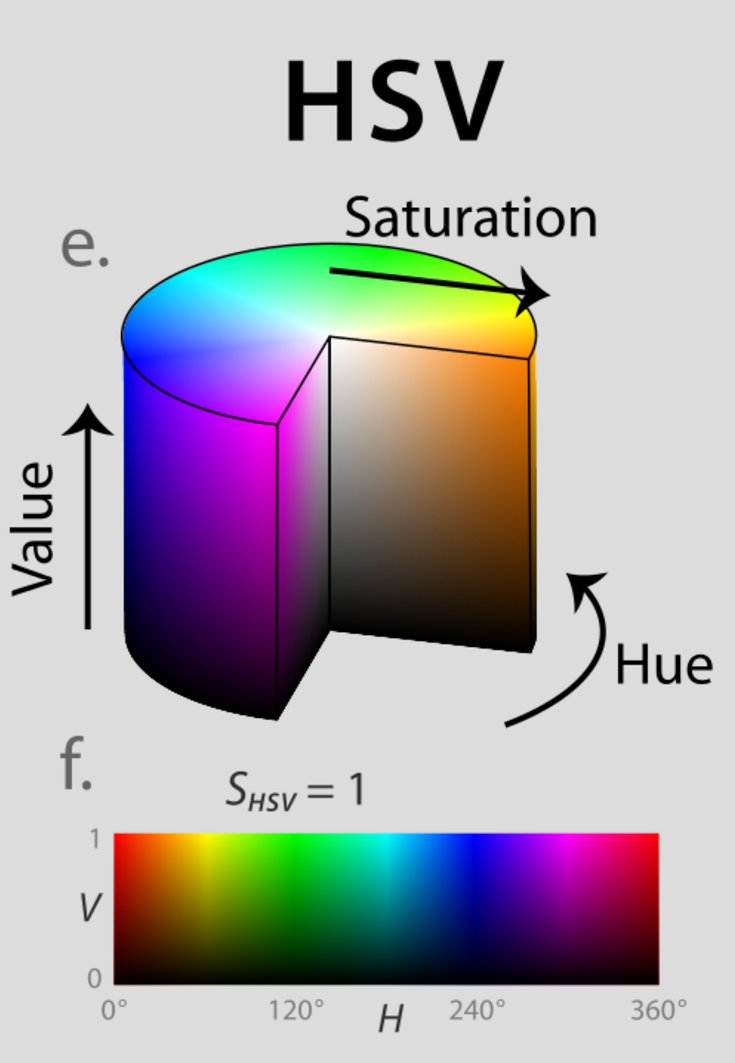
\includegraphics[width=8cm\textwidth]{HSV_cube}
    \caption{HSV Cube}
    \label{fig:HSV Cube}
\end{figure}

\newpage

Advantage of HSV color space is that Unlike RGB and CMYK, which are defined in relation to primary colors, HSV is defined in a way that is similar to how humans perceive color.

\begin{figure}[!hb]
    \centering
    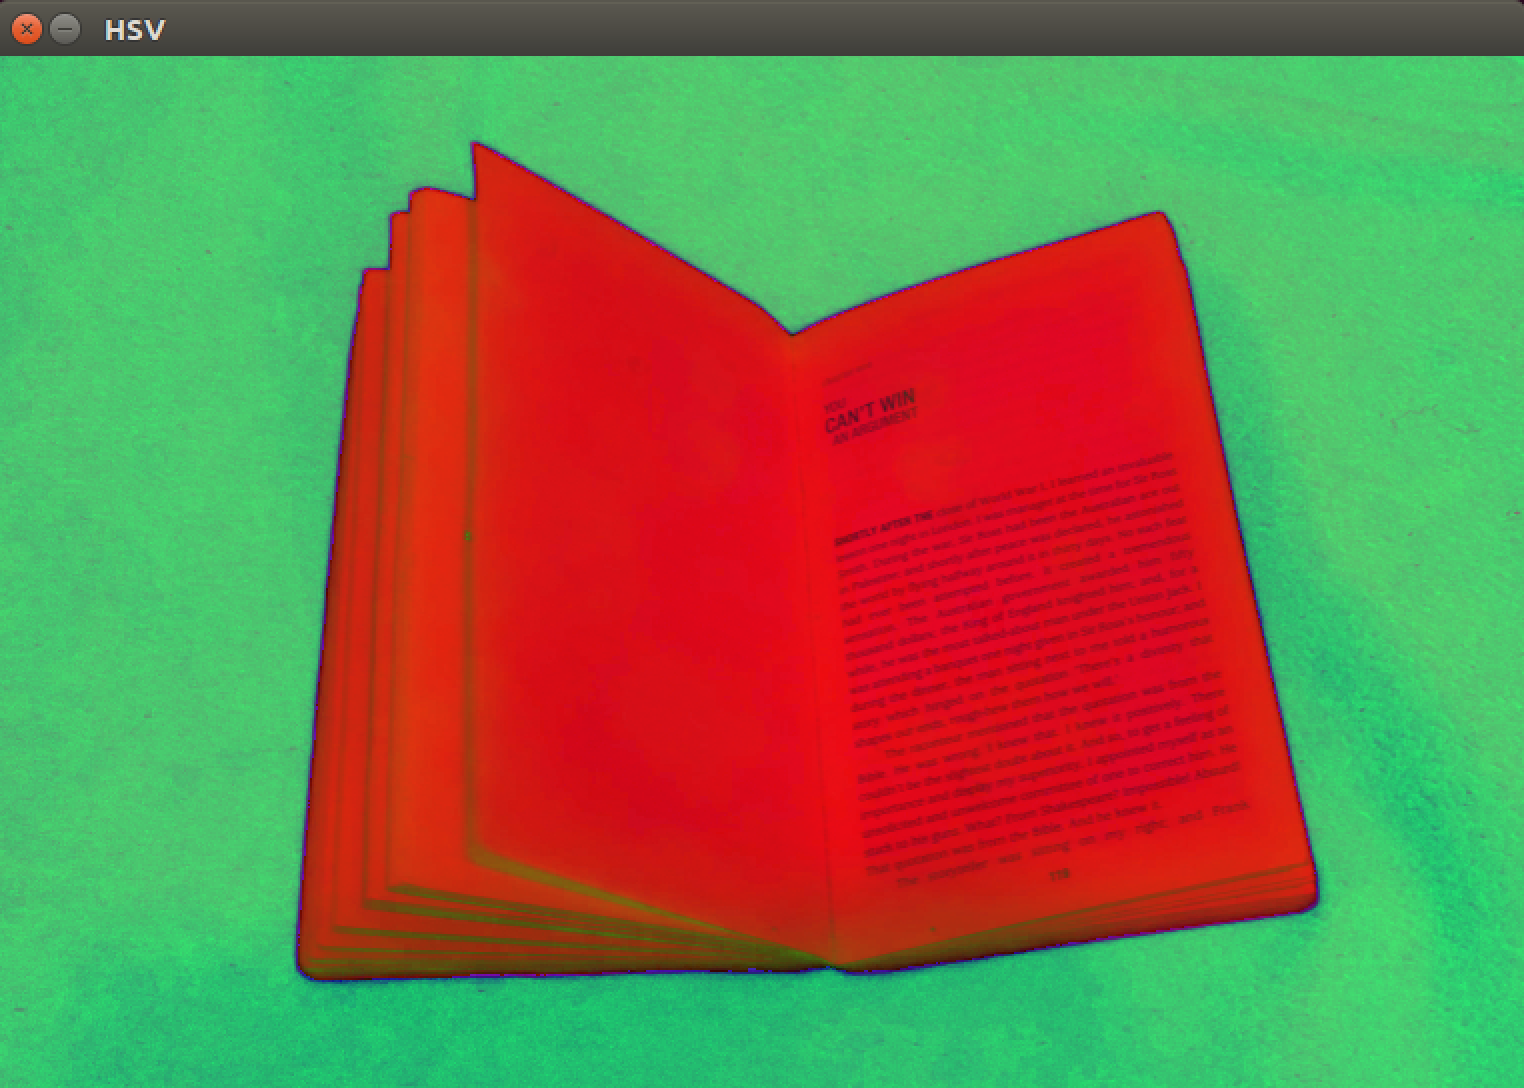
\includegraphics[width=15cm\textwidth]{hsv_colorspace}
    \caption{HSV Colorspace in our sample image}
    \label{fig:HSV Cube}
\end{figure}

\subsubsection{L*a*b* Color space}

Then there is the L*a*b* color space which is more tuned to how humans perceive color.

The Lab color space describes mathematically all perceivable colors in the three dimensions L for lightness and a and b for the color opponents green–red and blue–yellow. The terminology "Lab" originates from the Hunter 1948 color space.Nowadays "Lab" is frequently mis-used as abbreviation for CIEL*a*b* 1976 color space color space (also CIELAB); the asterisks/stars distinguish the CIE version from Hunter's original version. 

\newpage

OpenCV provides support for many, many different color spaces. And understanding how color is perceived by humans and represented by computers occupies an entire library of literature itself.

\begin{figure}[!hb]
    \centering
    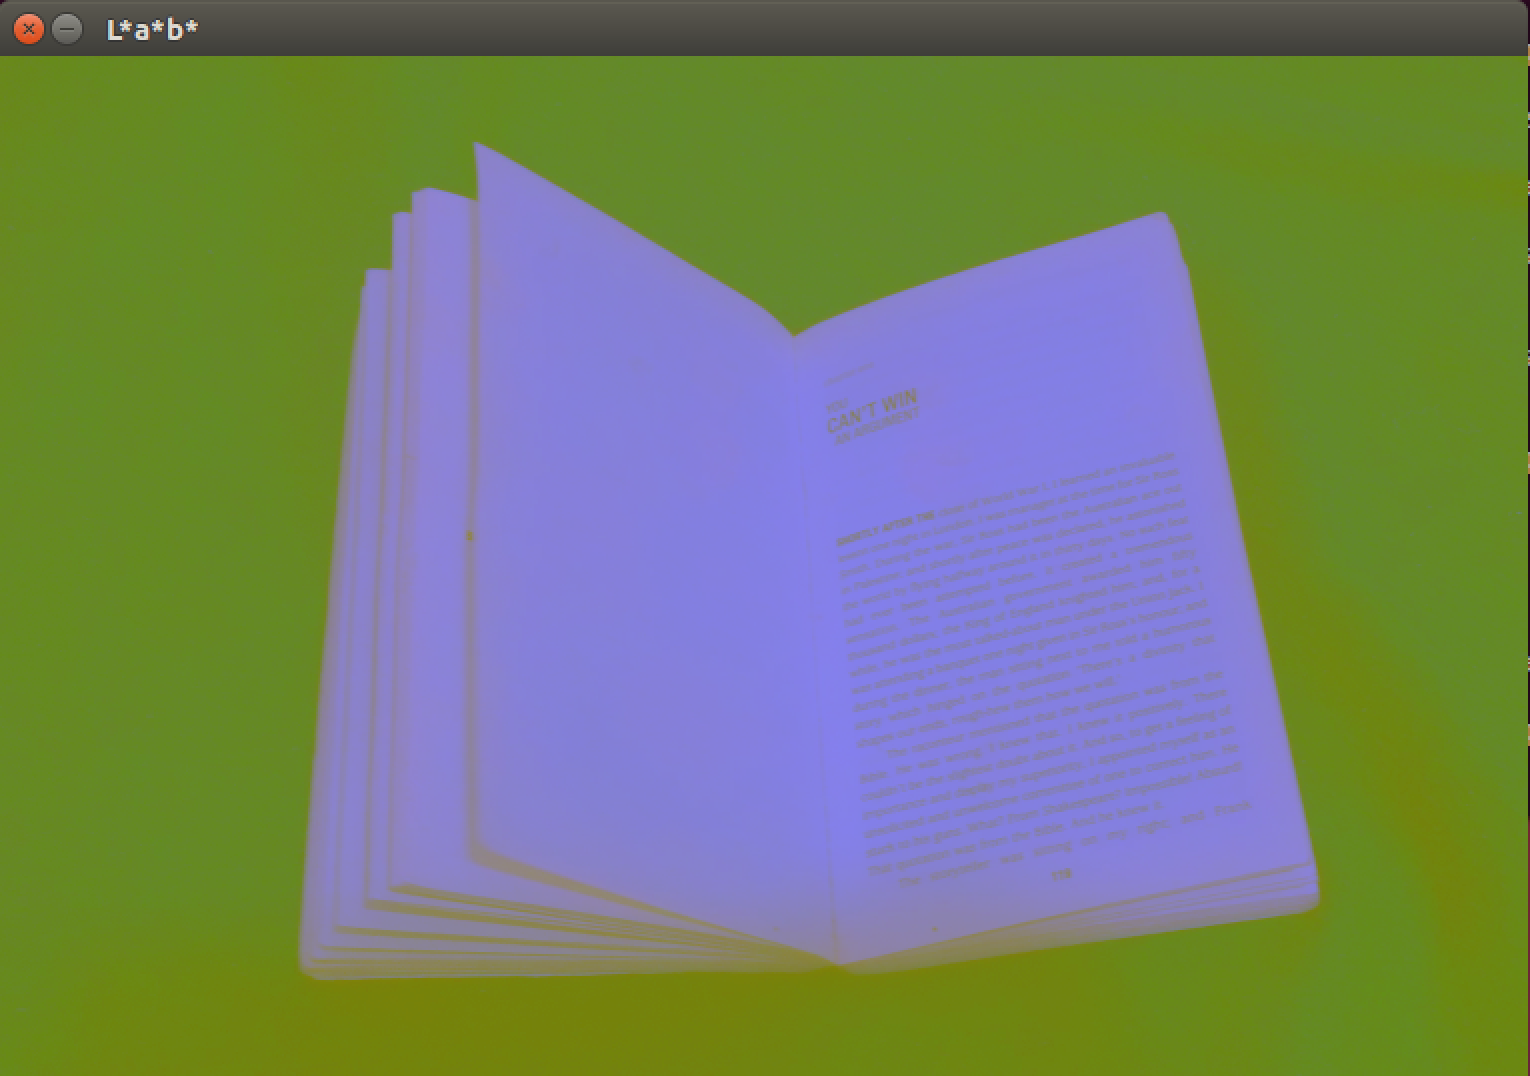
\includegraphics[width=15cm\textwidth]{lab_colorspace}
    \caption{L*a*b* Colorspace in our samle image}
    \label{fig:L*a*b* Colorspace}
\end{figure}

\subsubsection{Gray Color Space}

In photography and computing, a grayscale or greyscale digital image is an image in which the value of each pixel is a single sample, that is, it carries only intensity information. Images of this sort, also known as black-and-white, are composed exclusively of shades of gray, varying from black at the weakest intensity to white at the strongest.

Grayscale images are distinct from one-bit bi-tonal black-and-white images, which in the context of computer imaging are images with only two colors, black and white (also called bilevel or binary images). Grayscale images have many shades of gray in between.

Grayscale images are often the result of measuring the intensity of light at each pixel in a single band of the electromagnetic spectrum (e.g. infrared, visible light, ultraviolet, etc.), and in such cases they are monochromatic proper when only a given frequency is captured. But also they can be synthesized from a full color image; see the section about converting to grayscale.

The intensity of a pixel is expressed within a given range between a minimum and a maximum, inclusive. This range is represented in an abstract way as a range from 0 (total absence, black) and 1 (total presence, white), with any fractional values in between. This notation is used in academic papers, but this does not define what "black" or "white" is in terms of colorimetry.

Another convention is to employ percentages, so the scale is then from 0\% to 100\%. This is used for a more intuitive approach, but if only integer values are used, the range encompasses a total of only 101 intensities, which are insufficient to represent a broad gradient of grays. Also, the percentile notation is used in printing to denote how much ink is employed in halftoning, but then the scale is reversed, being 0\% the paper white (no ink) and 100\% a solid black (full ink).

In computing, although the grayscale can be computed through rational numbers, image pixels are stored in binary, quantized form. Some early grayscale monitors can only show up to sixteen (4-bit) different shades, but today grayscale images (as photographs) intended for visual display (both on screen and printed) are commonly stored with 8 bits per sampled pixel, which allows 256 different intensities (i.e., shades of gray) to be recorded, typically on a non-linear scale. The precision provided by this format is barely sufficient to avoid visible banding artifacts, but very convenient for programming because a single pixel then occupies a single byte.

\begin{figure}[!hb]
    \centering
    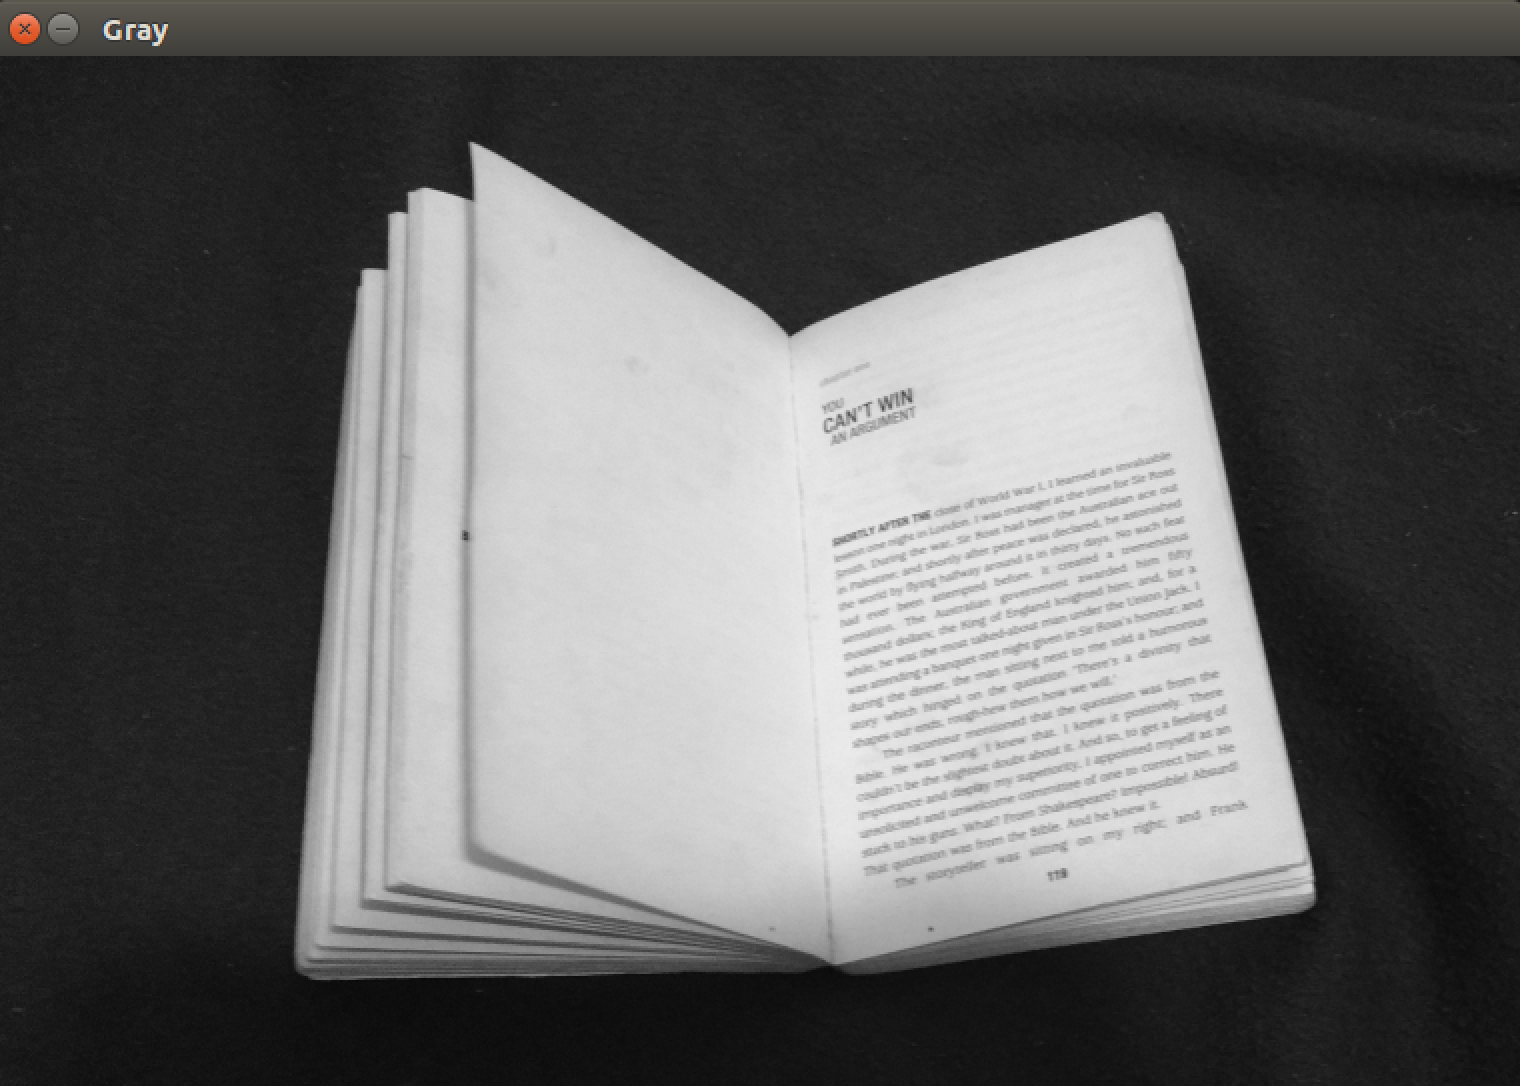
\includegraphics[width=15cm\textwidth]{gray_colorspace}
    \caption{Gray Colorspace in our sample image}
    \label{fig:Gray Colorspace}
\end{figure}

\begin{figure}[!hb]
    \centering
    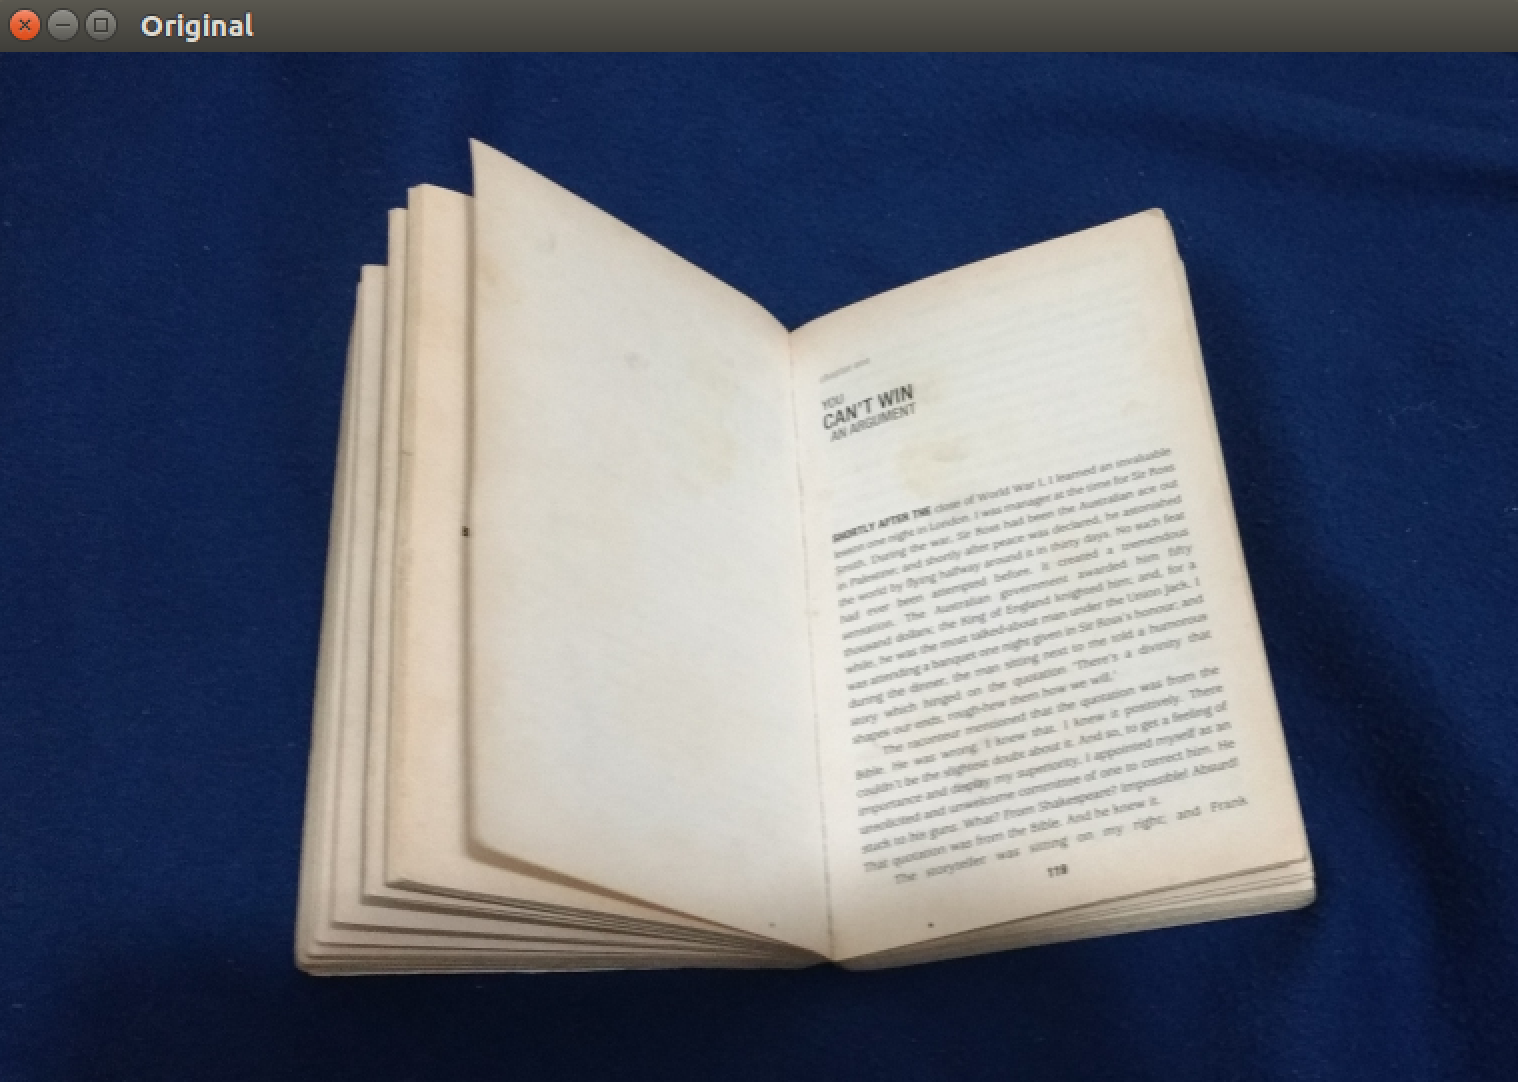
\includegraphics[width=15cm\textwidth]{normal_colorspace}
    \caption{Normal Colorspace in our sample image}
    \label{fig:Normal Colorspace}
\end{figure}

\newpage

\subsection{Channels}

A color image consists of multiple channels: a Red, a Green, and a Blue component. We have seen that we can access these components via indexing into NumPy arrays.

\begin{figure}[!hb]
    \centering
    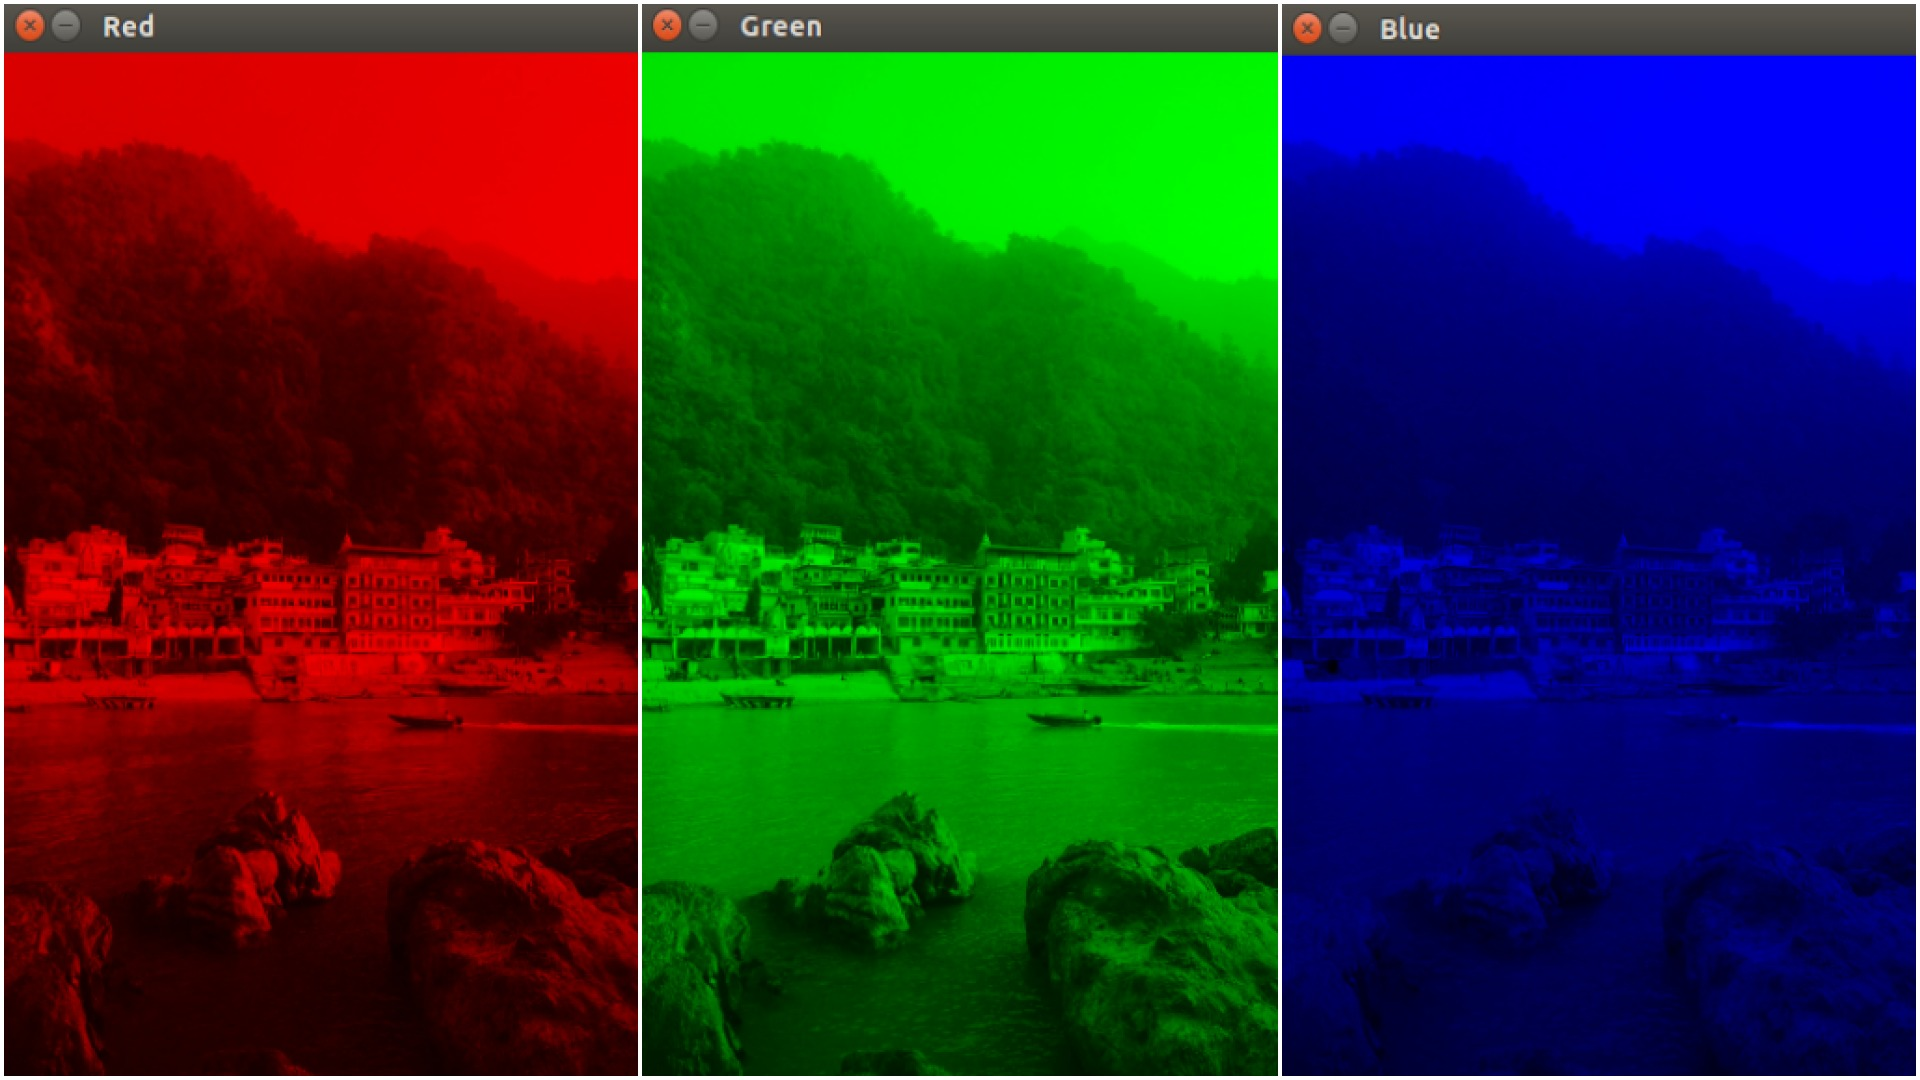
\includegraphics[width=15cm\textwidth]{channels}
    \caption{Red Green Blue Channels of the same image}
    \label{fig:Red Green Blue Channels of the same image}
\end{figure}

As you can see, the image has been divided up into three seperate channels mergin which you get the original image 

\begin{figure}[!hb]
    \centering
    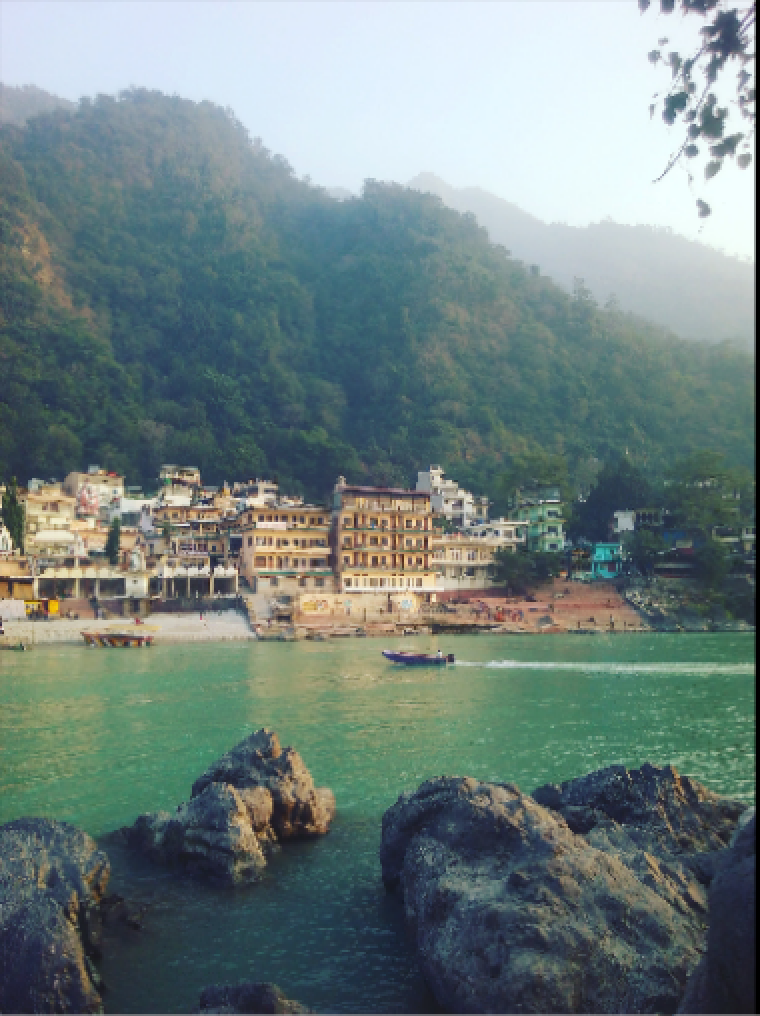
\includegraphics[width=6cm\textwidth]{og_channel}
    \caption{Red Green Blue Channels merged to form original image}
    \label{fig:Red Green Blue Channels of the same image}
\end{figure}

\subsection{Histograms}

So, what exactly is a histogram? A histogram represents the distribution of pixel intensities (whether color or gray- scale) in an image. It can be visualized as a graph (or plot) that gives a high-level intuition of the intensity (pixel value) distribution. We are going to assume a RGB color space in this example, so these pixel values will be in the range of 0 to 255.

When plotting the histogram, the X-axis serves as our “bins”. If we construct a histogram with 256 bins, then we are effectively counting the number of times each pixel
value occurs. In contrast, if we use only 2 (equally spaced) bins, then we are counting the number of times a pixel is in the range [0, 128) or [128, 255]. The number of pixels binned to the x-axis value is then plotted on the y-axis.

By simply examining the histogram of an image, you get a general understanding regarding the contrast, brightness, and intensity distribution.

\subsubsection{Using OpenCV to Build histograms}

We use cv2.calcHist() function to build our histograms

Here is the command to do so 

cv2.calcHist(images,channels,mask,histSize,ranges)

Let's quickly go through it once.

\begin{itemize}
    \item images: \par  This is the image that we want to compute a histogram for. Wrap it as a list: [myImage].
    \item channels: \par  A list of indexes, where we specify the index of the channel we want to compute a histogram for. To compute a histogram of a grayscale image, the list would be [0]. To compute a histogram for all three red, green, and blue channels, the channels list would be [0,1,2].
    \item mask: \par If a mask is provided, a histogram will be computed for masked pixels only. If we do not have a mask or do not want to apply one, we can just provide a value of None.
    \item histSize: \par This is the number of bins we want to use when computing a histogram. Again, this is a list, one for each channel we are computing a histogram for. The bin sizes do not all have to be the same. Here is an example of 32 bins for each channel: [32,32,32].
    \item ranges: \par The range of possible pixel values. Normally, this is [0, 256] for each channel, but if you are using a color space other than RGB (such as HSV), the ranges might be different.
\end{itemize}  

\subsection{Smoothing and blurring}

Blurring is what happens when your camera takes a picture out of focus. Sharper regions in the image lose their detail, normally as a disc/circular shape.

Practically, this means that each pixel in the image is mixed in with its surrounding pixel intensities. This “mixture” of pixels in a neighborhood becomes our blurred pixel.

While this effect is usually unwanted in our photographs, it’s actually quite helpful when performing image processing tasks.

In fact, many image processing and computer vision functions, such as thresholding and edge detection, perform better if the image is first smoothed or blurred.

\subsubsection{Averaging}

Averaging is a blurring method.

As the name suggests, we are going to define a k × k sliding window on top of our image, where k is always an odd number. This window is going to slide from left-to- right and from top-to-bottom. The pixel at the center of this matrix (and hence why we have to use an odd number, otherwise there would not be a true “center”) is then set to be the average of all other pixels surrounding it.

We call this sliding window a “convolution kernel” or just a “kernel”. 

In order to average blur an image, we use the cv2.blur() function. This function requires two arguments: the image we want to blur and the size of the kernel.

\subsubsection{Gaussian}

Next up, we are going to review Gaussian blurring. Gaussian blurring is similar to average blurring, but instead of using a simple mean, we are now using a weighted mean, where neighborhood pixels that are closer to the central pixel contribute more “weight” to the average.

The end result is that our image is less blurred, but more naturally blurred, than using the average method discussed in the previous section.

\subsubsection{Median}

Traditionally, the median blur method has been most effective when removing salt-and-pepper noise. This type of noise is exactly what it sounds like: imagine taking a photo- graph, putting it on your dining room table, and sprinkling salt and pepper on top of it. 

Using the median blur method, you could remove the salt and pepper from your image. When applying a median blur, we first define our kernel size k. Then, as in the averaging blurring method, we consider all pixels in the neighborhood of size k × k. But, unlike the averaging method, instead of replacing the central pixel with the average of the neighborhood, we instead replace the central pixel with the median of the neighborhood.

The reason median blurring is more effective at removing salt-and-pepper style noise from an image is that each central pixel is always replaced with a pixel intensity that exists in the image.

Methods such as averaging and Gaussian compute means or weighted means for the neighborhood – this average pixel intensity may or may not be present in the neighbor- hood. But by definition, the median pixel must exist in our neighborhood. By replacing our central pixel with a median rather than an average, we can substantially reduce noise.

\subsubsection{Bilateral}

The last method we are going to explore is bilateral blurring.

Thus far, the intention of our blurring methods have been to reduce noise and detail in an image; however, we tend to lose edges in the image.

In order to reduce noise while still maintaining edges, we can use bilateral blurring. Bilateral blurring accomplishes this by introducing two Gaussian distributions.

The first Gaussian function only considers spatial neighbors, that is, pixels that appear close together in the (x, y) coordinate space of the image. The second Gaussian then models the pixel intensity of the neighborhood, ensuring that only pixels with similar intensity are included in the actual computation of the blur.

Overall, this method is able to preserve edges of an image, while still reducing noise. The largest downside to this method is that it is considerably slower than its averaging, Gaussian, and median blurring counterparts.

\subsection{Thresholding}

Thresholding is the binarization of an image. In general, we seek to convert a grayscale image to a binary image, where the pixels are either 0 or 255.

A simple thresholding example would be selecting a pixel value p, and then setting all pixel intensities less than p to zero, and all pixel values greater than p to 255. In this way, we are able to create a binary representation of the image.

Normally, we use thresholding to focus on objects or areas of particular interest in an image. In the examples in the sections below, we will empty out our pockets and look at our spare change. Using thresholding methods, we’ll be able to find the coins in an image.

\subsubsection{Simple thresholding}

Applying simple thresholding methods requires human in- tervention. We must specify a threshold value T. All pixel intensities below T are set to 0. And all pixel intensities greater than T are set to 255.

We could also apply the inverse of this binarization by setting all pixels below T to 255 and all pixel intensities greater than T to 0.

\subsubsection{Adaptive thresholding}

One of the downsides of using simple thresholding meth- ods is that we need to manually supply our threshold value T. Not only does finding a good value of T require a lot of manual experiments and parameter tunings, it’s not very helpful if the image exhibits a lot of range in pixel intensities.
Simply put, having just one value of T might not suffice.

In order to overcome this problem, we can use adaptive thresholding, which considers small neighbors of pixels and then finds an optimal threshold value T for each neighbor. 

This method allows us to handle cases where there may be dramatic ranges of pixel intensities and the optimal value of T may change for different parts of the image.

\subsubsection{otsu and riddler-calvard}

Another way we can automatically compute the threshold value of T is to use Otsu’s method.

Otsu’s method assumes there are two peaks in the grayscale histogram of the image. In then tries to find an optimal value to separate these two peaks – thus our value of T.

While OpenCV provides support for Otsu’s method, I prefer the implementation by Luis Pedro Coelho in the mahotas package since it is more Pythonic.


\subsection{Gradients and edge detection}

Formally, edge detection embodies math- ematical methods to find points in an image where the brightness of pixel intensities changes distinctly.

The first thing we are going to do is find the “gradient” of the grayscale image, allowing us to find edge like regions in the x and y direction.

We’ll then apply Canny edge detection, a multi-stage pro- cess of noise reduction (blurring), finding the gradient of the image (utilizing the Sobel kernel in both the horizon- tal and vertical direction), non-maximum suppression, and hysteresis thresholding.


\section{Previous Work}

Many of the techniques of digital image processing \cite{wiki_digital_image_processing}, or digital picture processing as it often was called, were developed in the 1960s at the Jet Propulsion Laboratory, Massachusetts Institute of Technology, Bell Laboratories, University of Maryland, and a few other research facilities, with application to satellite imagery, wire-photo standards conversion, medical imaging, videophone, character recognition, and photograph enhancement. The cost of processing was fairly high, however, with the computing equipment of that era. That changed in the 1970s, when digital image processing proliferated as cheaper computers and dedicated hardware became available. Images then could be processed in real time, for some dedicated problems such as television standards conversion. As general-purpose computers became faster, they started to take over the role of dedicated hardware for all but the most specialized and computer-intensive operations.

With the fast computers and signal processors available in the 2000s, digital image processing has become the most common form of image processing and generally, is used because it is not only the most versatile method, but also the cheapest.

Digital image processing technology for medical applications was inducted into the Space Foundation Space Technology Hall of Fame in 1994.

In 2002 Raanan Fattel, introduced Gradient domain image processing, a new way to process images in which the differences between pixels are manipulated rather than the pixel values themselves.

\section{Motivation}

The purpose of detecting sharp changes in image brightness is to capture important events and changes in properties of the world. It can be shown that under rather general assumptions for an image formation model, discontinuities in image brightness are likely to correspond to:

\begin{itemize}
    \item discontinuities in depth
    \item discontinuities in surface orientation
    \item changes in material properties and
    \item variations in scene illumination
\end{itemize}


In the ideal case, the result of applying an edge detector to an image may lead to a set of connected curves that indicate the boundaries of objects, the boundaries of surface markings as well as curves that correspond to discontinuities in surface orientation. Thus, applying an edge detection algorithm to an image may significantly reduce the amount of data to be processed and may therefore filter out information that may be regarded as less relevant, while preserving the important structural properties of an image. If the edge detection step is successful, the subsequent task of interpreting the information contents in the original image may therefore be substantially simplified. However, it is not always possible to obtain such ideal edges from real life images of moderate complexity.

Edges extracted from non-trivial images are often hampered by fragmentation, meaning that the edge curves are not connected, missing edge segments as well as false edges not corresponding to interesting phenomena in the image – thus complicating the subsequent task of interpreting the image data.[4]

Edge detection is one of the fundamental steps in image processing, image analysis, image pattern recognition, and computer vision techniques.

The edges extracted from a two-dimensional image of a three-dimensional scene can be classified as either viewpoint dependent or viewpoint independent. A viewpoint independent edge typically reflects inherent properties of the three-dimensional objects, such as surface markings and surface shape. A viewpoint dependent edge may change as the viewpoint changes, and typically reflects the geometry of the scene, such as objects occluding one another.

A typical edge might for instance be the border between a block of red color and a block of yellow. In contrast a line (as can be extracted by a ridge detector) can be a small number of pixels of a different color on an otherwise unchanging background. For a line, there may therefore usually be one edge on each side of the line.

\section{Methods}

There are many methods for edge detection \cite{wiki_edge_detection}, but most of them can be grouped into two categories, search-based and zero-crossing based. The search-based methods detect edges by first computing a measure of edge strength, usually a first-order derivative expression such as the gradient magnitude, and then searching for local directional maxima of the gradient magnitude using a computed estimate of the local orientation of the edge, usually the gradient direction. The zero-crossing based methods search for zero crossings in a second-order derivative expression computed from the image in order to find edges, usually the zero-crossings of the Laplacian or the zero-crossings of a non-linear differential expression. As a pre-processing step to edge detection, a smoothing stage, typically Gaussian smoothing, is almost always applied (see also noise reduction).

The edge detection methods that have been published mainly differ in the types of smoothing filters that are applied and the way the measures of edge strength are computed. As many edge detection methods rely on the computation of image gradients, they also differ in the types of filters used for computing gradient estimates in the x- and y-directions.

A survey of a number of different edge detection methods can be found in (Ziou and Tabbone 1998); see also the encyclopedia articles on edge detection in Encyclopedia of Mathematics and Encyclopedia of Computer Science and Engineering.

\section{Objective}

The project aims to give a detailed comparison between the popularly used Edge detection techniques in Image processing. The motivation for this comparison arises from the fact that edge detection is one of the fundamental techniques used before many of the other image processing techniques and is used mainly in the pipe lining process. Which means that the output received from edge detection technique(s) would be used as the input of other image processing techniques.

This leads us down to the question as to which edge detection technique should one be using for his/her purpose.

We try to give a quantitative comparison of the various industry wide used edge detection techniques so that the reader who is thinking of applying edge detection for his work can make a clear and informed decision on which method would best suit his input and other requirements.

These edge detection techniques can be used widely in many problem sets. One such important use case would be to process handwritten notes. The very first task in processing hand written notes would be to detect the borders of the page which we are analysing. If the borders are detected, the next thing to do would be to pre-process the page for making it ready for other processes like Optical character recognition and likewise.

This paper dives deeper into the two
commonly used edge detection methods, namely

\begin{itemize}
    \item Canny Edge Detector and 
    \item Laplacian and Sobel Edge Detector.
\end{itemize}

 Both of them work with convolutions to achieve
the same end goal, i.e, finding edges. 

 \chapter{LITERATURE SURVEY}
\section{Approaches}
\ Image Segmentation \cite{researchgate_edge_det} is the process of partitioning a
digital image into multiple regions or sets of
pixels. Actually, partitions are different objects
in image which have the same texture or color. The result
of image segmentation is a set of regions that collectively
cover the entire image, or a set of contours extracted from
the image. All of the pixels in a region are similar with
respect to some characteristic or computed property, such
as color, intensity, or texture. Adjacent regions are
significantly different with respect to the same
characteristics. Edge detection is one of the most
frequently used techniques in digital image
processing. The boundaries of object surfaces in a
scene often lead to oriented localized changes in intensity
of an image, called edges. This observation combined
with a commonly held belief that edge detection is the
first step in image segmentation, has fueled a long search
for a good edge detection algorithm to use in image
processing. This search has constituted a principal
area of research in low level vision and has led to a
steady stream of edge detection algorithms published in
the image processing journals over the last two decades.
Even recently, new edge detection algorithms are
published each year. This paper will try to give a comparison of the various edge detection techniques released around.

Edge detection techniques transform images to edge
images benefiting from the changes of grey tones in the
images. Edges are the sign of lack of continuity, and
ending. As a result of this transformation, edge image is
obtained without encountering any changes in physical
qualities of the main image. Objects consist of
numerous parts of different color levels. In an image with
different grey levels, despite an obvious change in the 

1. Canny edge detection

2. Laplacian edge detection

3. Sobel edge detection

Edge Detection includes a variety of mathematical methods that aim at identifying points in a digital image at which the image brightness changes sharply or, more formally, has discontinuities.Most of the shape information of an image is enclosed in edges. So first we detect some edges in an image and by using these filters and then by enhancing those areas of image which contains edges, sharpness of the image will increase and image will become clearer.

\begin{equation}
f'(x)=df/dx(x) 
\label{eq:mkceqn}
\end{equation}  
the gradient of an image is defined as
\begin{equation}
\nabla I(u,v)=\begin{bmatrix}
\frac{\partial I}{\partial u}(u,v) \\
\frac{\partial I}{\partial v}(u,v)
\end{bmatrix}
\label{eq:sm}
\end{equation}
and the element consistent mass matrix is
\begin{equation}
[M^e]=\frac{\rho Al_e}{420}\begin{pmatrix}
156&22l_e &54&-13l_e\\
22l_e&4l_e^2&13l_e&-3l_e^2\\
54&13l_e&156&-22l_e\\
-13l_e&-3l_e^2&-22l_e&4l_e^2
\end{pmatrix}
\label{eq:cmm}
\end{equation}
\begin{equation}
[C]=\alpha[M]+\beta[K]
\end{equation}
A matrix equation with square matrices and vectors,
\begin{equation}
\begin{Bmatrix}
-M_1(t)\\
-V_1(t)\\
M_2(t)\\
V_2(t)\end{Bmatrix}=\begin{bmatrix}
D_{11}&D_{12}&D_{13}&D_{14}\\
D_{21}&D_{22}&D_{23}&D_{24}\\
D_{31}&D_{32}&D_{33}&D_{34}\\
D_{41}&D_{42}&D_{43}&D_{44}\end{bmatrix}\begin{Bmatrix}
v_1(t)\\
\theta_1(t)\\
v_2(t)\\
\theta_2(t)\end{Bmatrix}
\label{eq:D}
\end{equation}

The lower part is the 1-D image. The upper part is the intensity of each pixel of the 1-D image plotted as a graph. Blacks have a low intensity, so the graph curve is low. It reaches full height at the white end of the image. Note that the center of the curve has a steep slope - meaning there's an edge.

Looking for these peaks is exactly what gradient based edge detection methods do. We are not interested in what the actual colors are. If the change is steep enough, it is marked as an edge pixel. Though these methods work well, there's one drawback - how to decide what is a peak and what isn't? There has to be a certain threshold above which an edge is classified as a peak else it must be considered part of noise. Here's the next key idea: On the left (where the curve is rising), the slope is positive. On the right, the slope is negative. So there must exist a point where there is a zero crossing. That point is the edge's location. Edge detectors that are based on this idea are called Laplacian edge detectors.

\begin{figure}[h!]
    \centering
    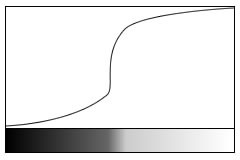
\includegraphics[width=10cm\textwidth]{intensity-curve}
    \caption{Intensity Curve}
    \label{fig:Intensity curve}
\end{figure}

\begin{figure}[h!]
    \centering
    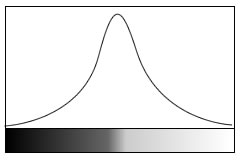
\includegraphics[width=10cm\textwidth]{first-derivative-curve}
    \caption{First Derivative curve}
    \label{fig:First Derivative curve}
\end{figure}
\begin{figure}[h!]
    \centering
    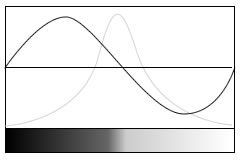
\includegraphics[width=10cm\textwidth]{second-derivative-curve}
    \caption{Second Derivative curve}
    \label{fig:Second Derivative curve}
\end{figure}

Now, all of this is for 1-D images. It turns out that all of this holds for 2-D images as well. So we can simply use these results and try them on actual images. Another thing is - these are based on continuous images. For us, that is never the case. So we'll have to approximate these derivatives based on the pixelated data that we do have. This is done with the help of convolutions.

 \section{Canny edge detection algorithm}
\ It is a popular edge detection algorithm developed by John F. Canny in 1986. It is a multi-stage algorithm divided into the following steps:



1. \underline{Noise Reduction}- The first step is to remove  any kind of noise from the image before actual edge detection. It is done with the help of a Gaussian filter.
\begin{itemize}
\item Gaussian filter - Since all edge detection results are easily affected by image noise, it is essential to filter out the noise to prevent false detection caused by noise. To smooth the image, a Gaussian filter is applied to convolve with the image. This step will slightly smooth the image to reduce the effects of obvious noise on the edge detector.
\begin{equation}
H_{ij}=\frac{1}{2\pi\sigma^2}exp(-\frac{(i-(k+1))^2)+(j-(k+1))^2}{2\sigma^2})
\label{eq:mkceqn}
\end{equation} 
\end{itemize}

2. \underline{Finding Intensity Gradient} - The smoothened
image is then filtered with a Sobel Kernel in both horizontal and vertical directions to get the first set of derivatives. From this process we find out the edge gradient and direction of each pixel.The edge detection operator returns a value for the first derivative in the horizontal direction (Gx) and the vertical direction (Gy). From this the edge gradient and direction can be d\begin{equation}
G=\sqrt{G_{x}^2+G_{x}^2}
\label{eg:mkceqn}
\end{equation}


3. \underline{Non-maximum Suppression} - After finding out the edge gradient and the direction of each pixel, a full scan of the image is done to remove any unwanted pixels which may not constitute the edge. This involves checking every pixel to its local maximum in its neighbourhood in the direction of gradient.Non-maximum suppression is an edge thinning technique.

\begin{figure}[h!]
    \centering
    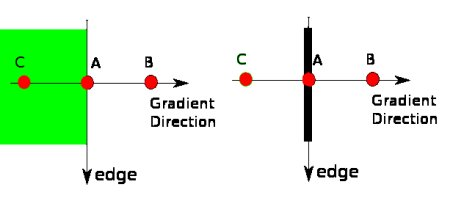
\includegraphics[width=10cm\textwidth]{nms}
    \caption{Non-maximum suppression}
    \label{fig:Non-maximum suppression}
\end{figure}

Non-Maximum suppression is applied to "thin" the edge. After applying gradient calculation, the edge extracted from the gradient value is still quite blurred.At every pixel, it suppresses the edge strength of the center pixel (by setting its value to 0) if its magnitude is not greater than the magnitude of the two neighbors in the gradient direction. For example,
\begin{itemize}
\item if the rounded gradient angle is 0{\degree} (i.e. the edge is in the north-south direction) the point will be considered to be on the edge if its gradient magnitude is greater than the magnitudes at pixels in the east and west directions,
\end{itemize}
\begin{itemize}
\item if the rounded gradient angle is 90{\degree} (i.e. the edge is in the east-west direction) the point will be considered to be on the edge if its gradient magnitude is greater than the magnitudes at pixels in the north and south directions,
\end{itemize}
\begin{itemize}
\item if the rounded gradient angle is 135{\degree} (i.e. the edge is in the northeast-southwest direction) the point will be considered to be on the edge if its gradient magnitude is greater than the magnitudes at pixels in the north west and south east directions,
\end{itemize}
\begin{itemize}
\item if the rounded gradient angle is 45{\degree} (i.e. the edge is in the north west-south east direction) the point will be considered to be on the edge if its gradient magnitude is greater than the magnitudes at pixels in the north east and south west directions.
\end{itemize}
In more accurate implementations, linear interpolation is used between the two neighbouring pixels that straddle the gradient direction. For example, if the gradient angle is between 45 and 90, interpolation between gradients at the north and north east pixels will give one interpolated value, and interpolation between the south and south west pixels will give the other value.The gradient magnitude at the central pixel must be greater than both of these for it to be marked as an edge.

4. \underline{Hysteresis Thresholding} - At this stage, all edges are pitted against an established max-value and
min-value. Any edge with intensity gradient higher than the max-value are assumed to be edges and ones that are lower will be discarded. It is decided based on how closely connected are the edges in question to the max-value and
the min-value.

\begin{figure}[h!]
    \centering
    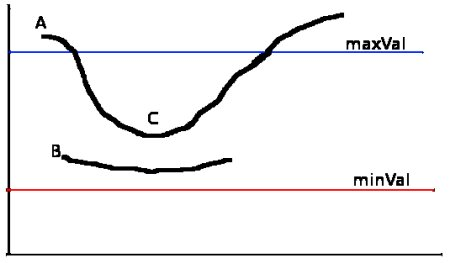
\includegraphics[width=10cm\textwidth]{hysteresis}
    \caption{Hysteresis}
    \label{fig:Hysteresis}
\end{figure}

5. \underline{Double threshold} - After application of non-maximum suppression, remaining edge pixels provide a more accurate representation of real edges in an image. However, some edge pixels remain that are caused by noise and color variation. In order to account for these spurious responses, it is essential to filter out edge pixels with a weak gradient value and preserve edge pixels with a high gradient value. This is accomplished by selecting high and low threshold values. If an edge pixel's gradient value is higher than the high threshold value, it is marked as a strong edge pixel. If an edge pixel's gradient value is smaller than the high threshold value and larger than the low threshold value, it is marked as a weak edge pixel. If an edge pixel's value is smaller than the low threshold value, it will be suppressed.

So the usual work flow \cite{drexel_canny} of working with Canny edge detection algorithm would be to follow the steps as

\begin{enumerate}
    \item Apply a Gaussian blur 
    \\
    \begin{itemize}
        \item First necessary variables are declared and some are initialized. Then a Gaussian blur is applied. To do this a 5x5 mask is passed over the image. Each pixel is redefined as the sum of the pixel values in its 5x5 neighborhood times the corresponding Gaussian weight, divided by the total weight of the whole mask.
    \end{itemize}
    \begin{figure}[h!]
        \centering
        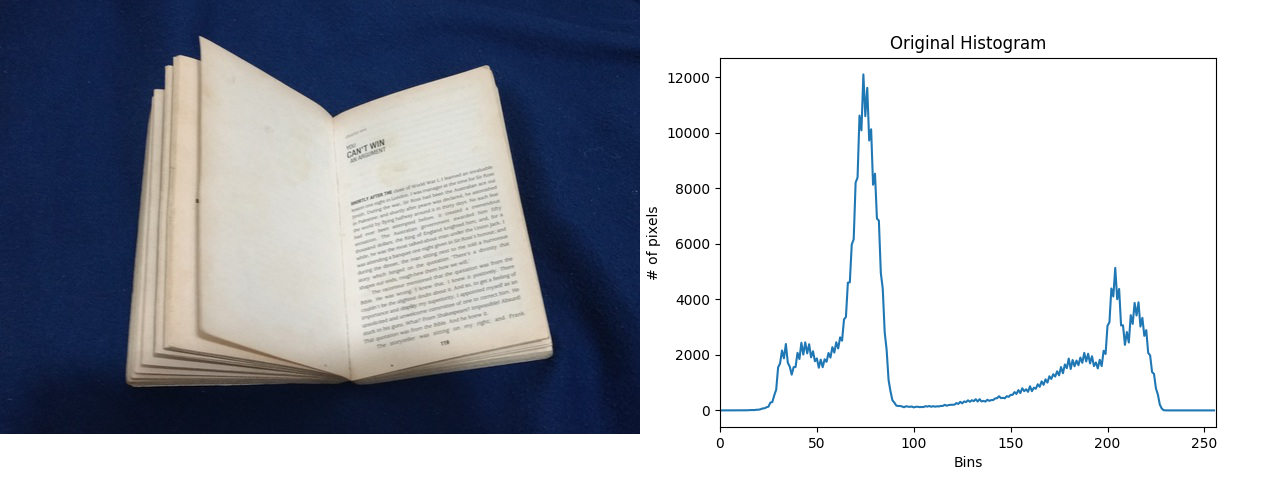
\includegraphics[width=15cm\textwidth]{win_frnds_blue_orig_hist}
        \caption{Original input image}
        \label{fig:Original input image}
    \end{figure}
    \begin{figure}[h!]
        \centering
        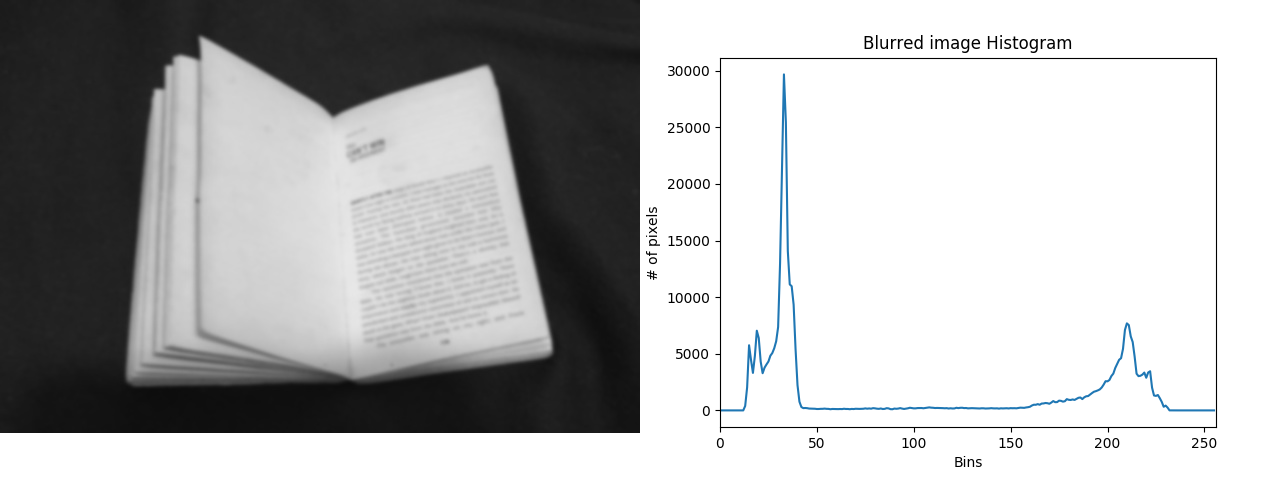
\includegraphics[width=15cm\textwidth]{win_frnds_blue_blurred_grayed_hist}
        \caption{Applying a Gaussian blur over grayscaled image}
        \label{fig:Applying Gaussian blur}
    \end{figure}
    \item Find edge gradient strength and direction
    \\
    \begin{itemize}
        \item The next step is to use Sobel masks to find the edge gradient strength and direction for each pixel. First the Sobel masks are applied to the 3x3 pixel neighborhood of the current pixel, in both the x and y directions. Then the sum of each mask value times the corresponding pixel is computed as the Gx and Gy values, respectively. The square root of Gx squared plus Gy squared equals the edge strength. The inverse tangent of Gx / Gy yields the edge direction. The edge direction is then approximated to one of four possible values that make up the possible directions an edge could be in an image made up of a square pixel grid. This edge direction is then stored in the array edgeDir[row][col] and the gradient strength is stored in the array gradient[row][col].
    \end{itemize}
    \item Trace along the edges
    \\
    \begin{itemize}
        \item The next step is to actually trace along the edges based on the previously calculated gradient strengths and edge directions. Each pixel is cycled through using two nested for loops. If the current pixel has a gradient strength greater than the defined upperThreshold, then a switch is executed. The switch is determined by the edge direction of the current pixel. It stores the row and column of the next possible pixel in that direction and then tests the edge direction and gradient strength of that pixel. If it has the same edge direction and a gradient strength greater than the lowerThreshold, that pixel is set to white and the next pixel along that edge is tested. In this manner any significantly sharp edge is detected and set to white while all other pixels are set to black.
    \end{itemize}
    \begin{figure}[h!]
        \centering
        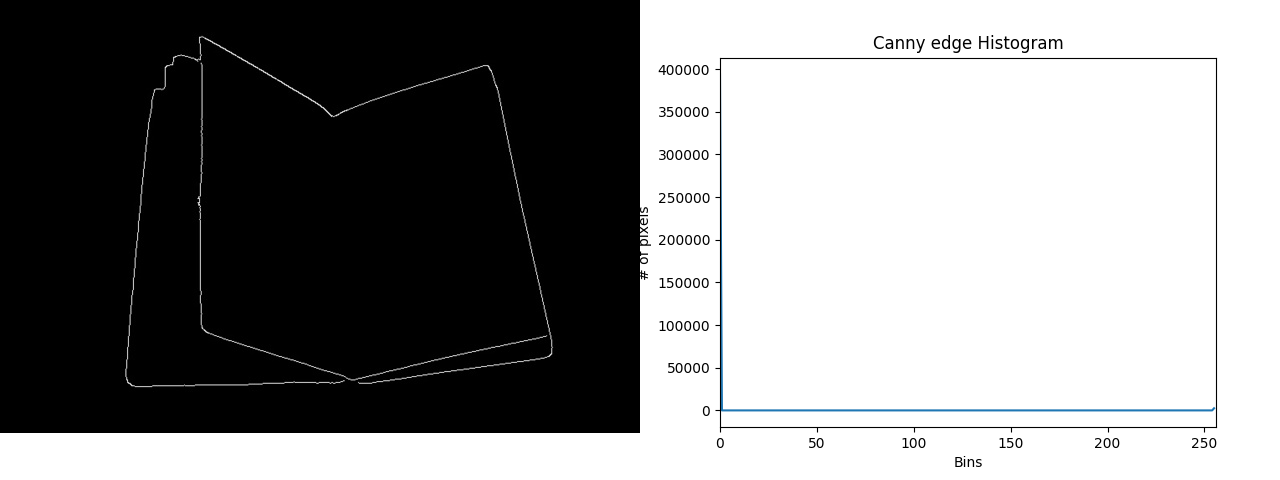
\includegraphics[width=15cm\textwidth]{win_frnds_blue_canny_hist}
        \caption{Canny Edges detected in input image}
        \label{fig:Canny Edges detected in input image}
    \end{figure}
    \item Suppress non-maximum edges
    \\
    \begin{itemize}
        \item The last step is to find weak edges that are parallel to strong edges and eliminate them. This is accomplished by examining the pixels perpendicular to a particular edge pixel, and eliminating the non-maximum edges. The code used is very similar to the edge tracing code.
    \end{itemize}
\end{enumerate}

\section{Improvement on Canny edge detection}
Traditional canny edge detection provides relatively simple but precise methodology for edge detection problem, with the more demanding requirements on the accuracy and robustness on the detection, the traditional algorithm can no longer handle the challenging edge detection task. The main defects of the traditional algorithm can be summarized as following:

1. Gaussian filter is applied to smooth out the noise, but it will also smooth the edge, which is considered as the high frequency feature. This will increase the possibility to miss weak edges, and the appearance of isolated edges in the result.

2. For the gradient amplitude calculation, the old canny edge detection algorithm uses center in a small 2x2 neighborhoods window to calculate the finite difference mean value to represent the gradient amplitude. This method is sensitive to noise and can easily detect fake edges and lose real edges.

3. In traditional canny edge detection algorithm, there will be two fixed global threshold values to filter out the false edges. However, as the image gets complex, different local areas will need very different threshold values to accurately find the real edges. In addition, the global threshold values are determined manually through experiments in the traditional method, which leads to complexity of calculation when large number of different images needs to be dealt with.

3. The result of the traditional detection cannot reach a satisfactory high accuracy of single response for each edge- multi-point responses will appear.



\section{Laplacian edge detection algorithm}
\ This is a very popular
algorithm for line and edge detection and also for
other complex algorithms to build-up their systems.
It involves the following steps:

1. \underline{Convert image to grey-scale format} - A coloured picture could also be done by splitting all the
channels and then merging them back but between this and the grey-scaled version there isn't much difference after.

2. \underline{Calculate Laplacian} - Laplacian is a derivative operator; its uses highlight gray level discontinuities in an image and try to deemphasize regions with slowly varying gray levels. This operation in result produces such images which have grayish edge lines and other discontinuities on a dark background. This produces inward and outward edges in an image

\begin{figure}[h!]
    \centering
    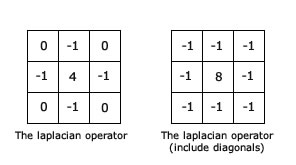
\includegraphics[width=12cm\textwidth]{laplacian-kernel}
    \caption{Laplacian kernel example}
    \label{fig:Laplacian kernel}
\end{figure}

The important thing is how to apply these filters onto image. We can't apply both the positive and negative Laplacian operator on the same image. we have to apply just one but the thing to remember is that if we apply positive Laplacian operator on the image then we subtract the resultant image from the original image to get the sharpened image. Similarly if we apply negative Laplacian operator then we have to add the resultant image onto original image to get the sharpened image.
It calculates the Laplacian  of an image by only one kernel filter, which finally gives the edges of the image in a much noisier way than the Canny method. The difference between Laplacian and other operators is that unlike other operators Laplacian didn't take out edges in any particular direction but it take out edges in following classification.

\begin{figure}[h!]
    \centering
    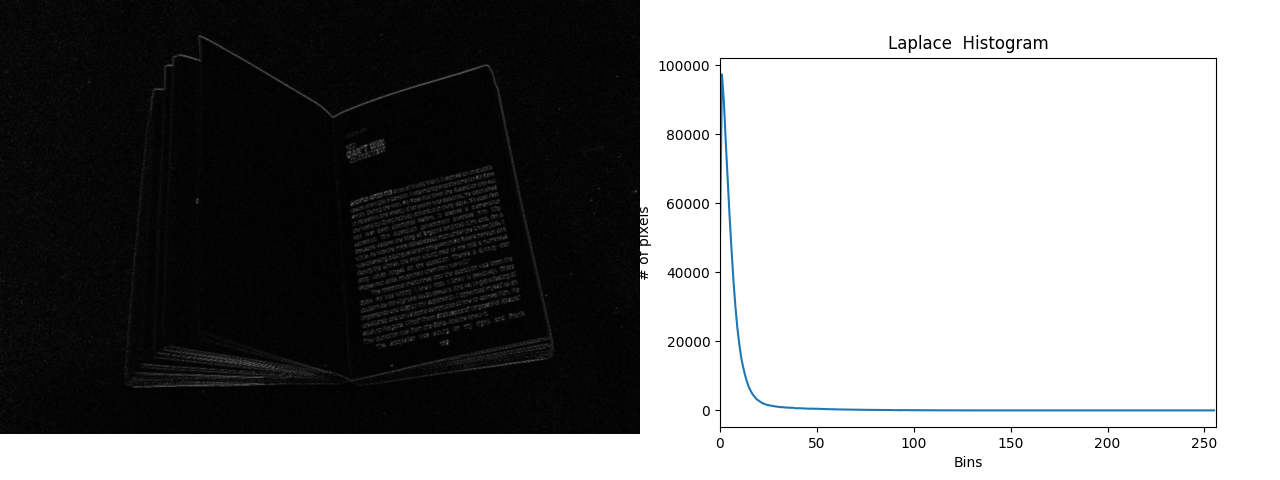
\includegraphics[width=15cm\textwidth]{laplace_hist}
    \caption{Laplacian Edges detected in given image}
    \label{fig:Laplacian Edges detected in given image}
\end{figure}

1. Inward Edges

2. Outward Edges

\section{Sobel edge detection algorithm}  

The sobel operator is very similar to Prewitt operator. It is also a derivate mask and is used for edge detection. Like Prewitt operator sobel operator is also used to detect two kinds of edges in an image:

1. Vertical direction

2. Horizontal direction

\underline{Difference with Prewitt Operator}

The major difference is that in sobel operator the coefficients of masks are not fixed and they can be adjusted according to our requirement unless they do not violate any property of derivative masks.The major difference is that in sobel operator the coefficients of masks are not fixed and they can be adjusted according to our requirement unless they do not violate any property of derivative masks.
This mask works exactly same as the Prewitt operator vertical mask. There is only one difference that is it has "2" and "-2" values in center of first and third column. When applied on an image this mask will highlight the vertical edges.

\begin{figure}[h!]
    \centering
    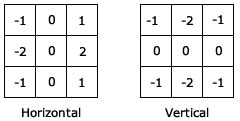
\includegraphics[width=10cm\textwidth]{sobel-kernels1}
    \caption{Sobel kernel example}
    \label{fig:Sobel kernel}
\end{figure}

It is a well-known algorithm used for contour detection. Sobel operation is a combined Gaussian smoothing along with differentiation operation, so it is somewhat more resistant to noise in which one can control the direction of the directives and also the kernel size. For sizes less than -1, a Scharr filter gives better result than the sobel filter.

\begin{figure}[h!]
    \centering
    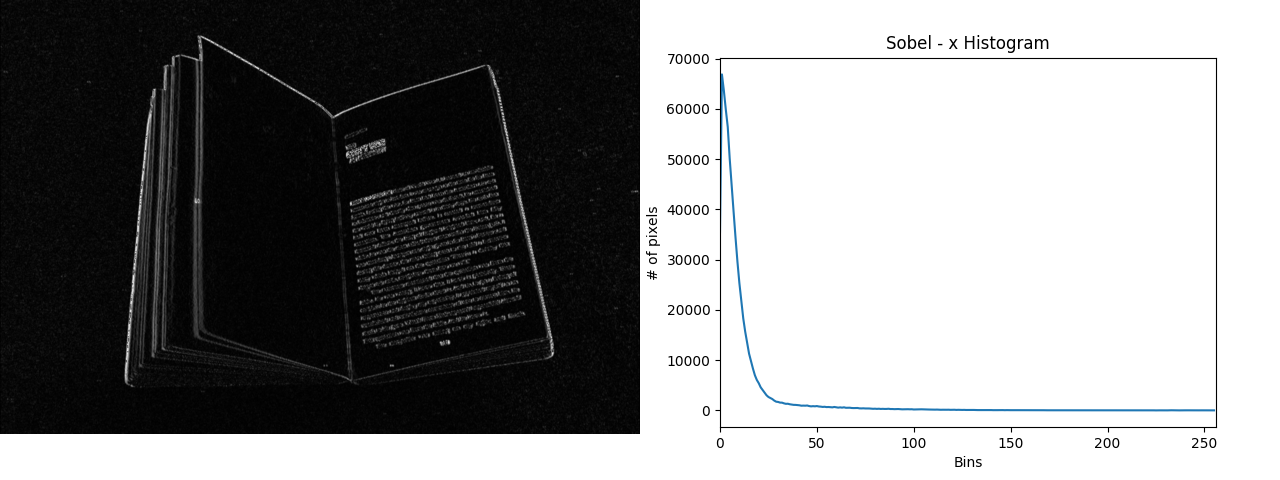
\includegraphics[width=15cm\textwidth]{sobel_x_combined_hist}
    \caption{Sobel's x-axis output with histogram}
    \label{fig:Sobel's x-axis output with histogram}
\end{figure}
\begin{figure}[h!]
    \centering
    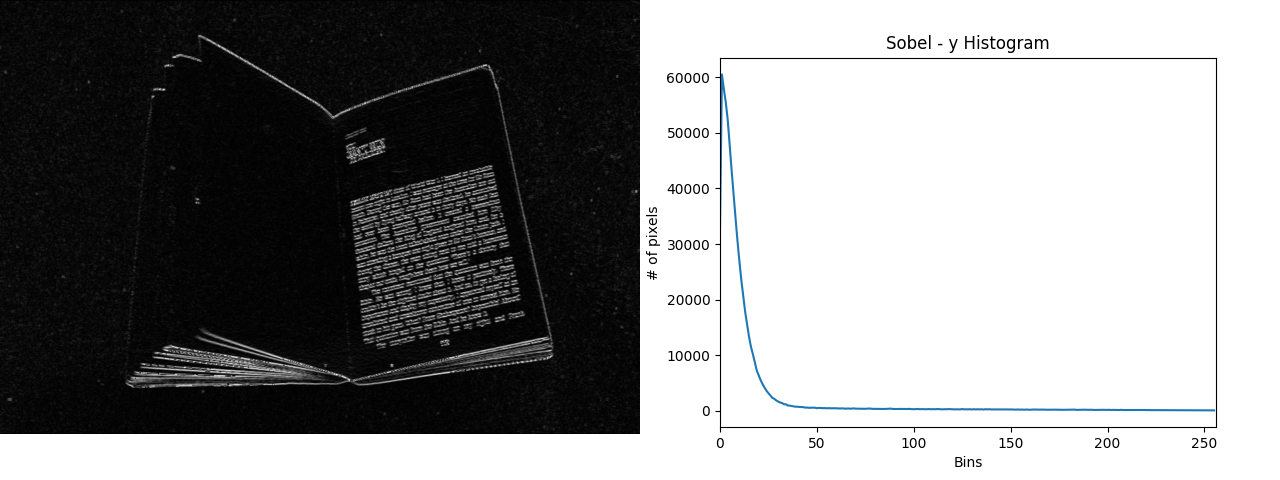
\includegraphics[width=15cm\textwidth]{sobel_y_combined_hist}
    \caption{Sobel's y-axis output with histogram}
    \label{fig:Sobel's y-axis with histogram}
\end{figure}
\begin{figure}[h!]
    \centering
    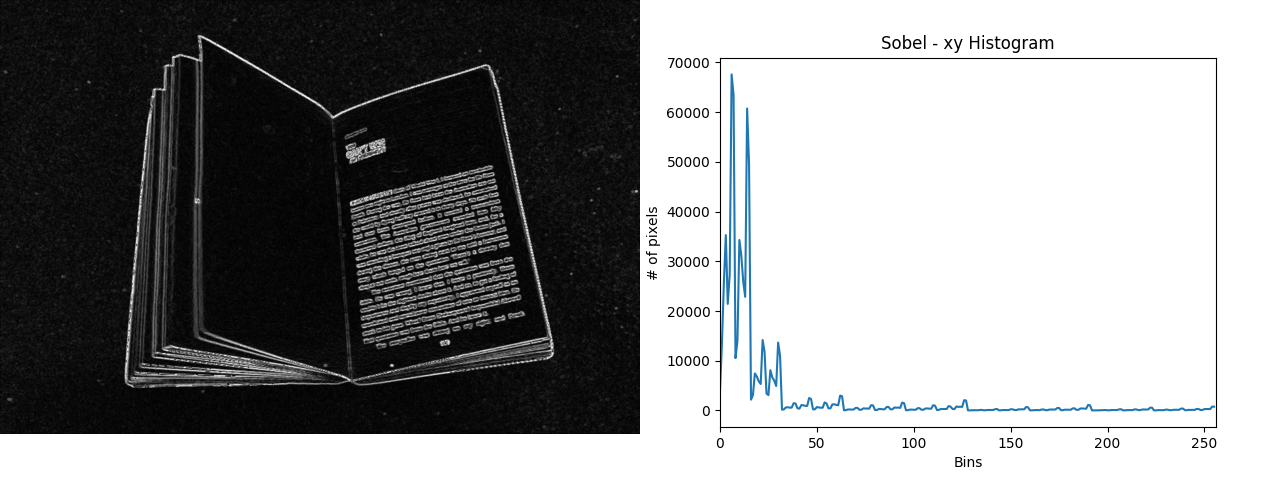
\includegraphics[width=15cm\textwidth]{sobel_xy_combined_hist}
    \caption{Sobel's x and y-axes combined output with histogram}
    \label{fig:Sobel's x and y-axes combined output with histogram}
\end{figure}

In digital image, the so-called edge is a collection of the pixels whose gray value has a step or roof change, and it also refers to the part where the brightness of the image local area changes significantly. The gray profile in this region can generally be seen as a step. That is, in a small buffer area, a gray value rapidly changes to another whose gray value is largely different with it. Edge widely exists between objects and  backgrounds, objects and objects, primitives and primitives. The edge of an object is reflected in the discontinuity of the gray. Therefore, the general method of edge detection is to study the changes of a single image pixel in a gray area, use the variation of the edge neighboring first order or second-order to detect the edge. This method is used to refer as local operator edge detection method. Edge detection is mainly the measurement, detection and location of the changes in image gray. Image edge is the most basic features of the image. When we observe the objects, the clearest part we see firstly is edge and line. According to the composition of the edge and line, we can know the object structure. Therefore, edge extraction is an important technique in graphics processing and feature extraction. The basic idea of edge detection is as follows: First, use edge enhancement operator to highlight the local edge of the image. Then, define the pixel "edge strength" and set the threshold to extract the edge point set. However, because of the noise and the blurring image, the edge detected may not be continuous. So, edge detection includes two contents. 
First is using edge operator to extract the edge point set. Second is removing some of the edge points from the edge point set, filling it with some another and linking the obtained edge point set into lines. 

\begin{equation}
f'(x)=df/dx(x) 
\label{eq:mkceqn}
\end{equation} 

\section{Improved Algorithm}
% http://islab.ulsan.ac.kr/files/announcement/328/An%20Improved%20Sobel%20Edge%20Detection.pdf
The advantage of Sobel edge operand is its smoothing
effect to the random noises in the image. And because it is
the differential separated by two rows or two columns, so the
edge elements on both sides have been enhanced and make
the edge seems thick and bright. Sobel operator is a gradient
operator. The first derivative of a digital image is based on a
variety of two-dimensional gradient approximation, and
generates a peak on the first derivative of the image, or
generates a zero-crossing point on the second derivative.
Calculate the magnitude and the argument value of the image
horizontal and vertical first-order or second-order gradients,
at last calculate modulus maxima along the angular direction
and obtain the edge of the image. But when the image has
lots of white Gaussian noises, it is very difficult to get the
peak value of the first derivative, the reason is because that
the noise points and the useful signals mix up. Therefore this
paper combines Sobel operator and soft-threshold wavelet
de-noising. The core idea of the algorithm is:

1. Do wavelet decomposition to the image matrix
and get the wavelet coefficients with noises.

2. Process the wavelet coefficients HL, LH and HH
obtained by the decomposition, and keep the lowfrequency
coefficients unchanging.

3. Select an appropriate threshold to remove
Gaussian white noise signals.

4. Do inverse wavelet transformation to the image
matrix and get the image matrix after de-noising.

5. Custom template edge coefficient according to the
Sobel operator template.

6. After given Sobel edge detection operator
template, convolute on every pixel of the image
using this template, get the gradient of this point,
and the gradient amplitude is the output of this
point. At last we get the edge detection image.
 

%%%%%%%%%%%%%%%%%%%%%%%%%%%%%%%%%%%%%%%%%%%%%%%%%%%%%%%%%%%%
% system design

% The System Design Document describes the system requirements, operating environment, system and subsystem architecture, files and database design, input formats, output layouts, human-machine interfaces, detailed design, processing logic, and external interfaces

\chapter{System Design}

\section{System Architecture}

\subsection{System Hardware Requirements}

After installation, connect to the server with SSH or a local terminal and execute the following commands to install OpenCV.

We tested it with the following hardware configurations

\begin{itemize}
    \item Ubuntu x86 64-bit 16.04 desktop edition.
    \item 2GB RAM
    \item 50GB Hard disk space
    \item 2MHZ processor
\end{itemize}

\section{Software Dependencies}

There are various packages and bits of software which are required for building OpenCV version 3.0.0 from scratch.

\subsection{Developer and compile tools}

\begin{itemize}
    \item build-essential
    \item cmake
    \item git
    \item pkg-config
    \item unzip
\end{itemize}

\subsection{Libraries for various image formats}

\begin{itemize}
    \item libjpeg8-dev
    \item libtiff4-dev
    \item libjasper-dev
    \item libpng12-dev
\end{itemize}

\subsection{Libraries for various video formats}

\begin{itemize}
    \item libavcodec-dev
    \item libavformat-dev
    \item libswscale-dev
    \item libv4l-dev
\end{itemize}

\subsection{GTK for OpenCV GUI}

\begin{itemize}
    \item libgtk2.0-dev
\end{itemize}

\subsection{Packages used for optimization in OpenCV}

\begin{itemize}
    \item libatlas-base-dev
    \item gfortran
\end{itemize}

\subsection{Python virtual environment}

Virtualenv is a tool which allows us to make isolated python environments. How does making isolated python environments help us ? Imagine you have an application that needs version 2 of a LibraryBar, but another application requires version 2. How can you use and develop both these applications? If you install everything into /usr/lib/python2.7/site-packages (or whatever your platform’s standard location is), it’s easy to end up in a situation where you unintentionally upgrade an application that shouldn’t be upgraded.

A Virtual Environment is a tool to keep the dependencies required by different projects in separate places, by creating virtual Python environments for them. It solves the “Project X depends on version 1.x but, Project Y needs 4.x” dilemma, and keeps your global site-packages directory clean and manageable.

The dependencies for Python using OpenCV version 3.0.0 are 

\begin{itemize}
    \item numpy v1.12.0
    \item Pillow v4.0.0
    \item scipy v0.18.1
\end{itemize}

\begin{figure}[h]
    \centering
    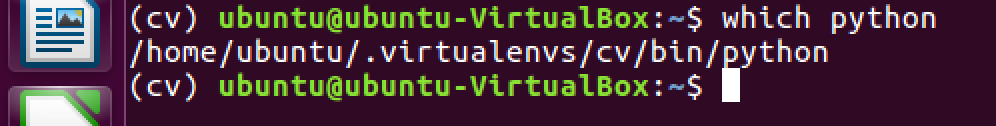
\includegraphics[width=15cm\textwidth]{virtualenv}
    \caption{Using the python version installed inside the virtual environment}
    \label{fig:virtual env}
\end{figure}

In the figure above, you can see that we are using the python version installed inside the virtualenv and not the default python stated inside our system PATH. This helps in managing dependencies better and avoiding any conflicts.

\begin{figure}[h]
    \centering
    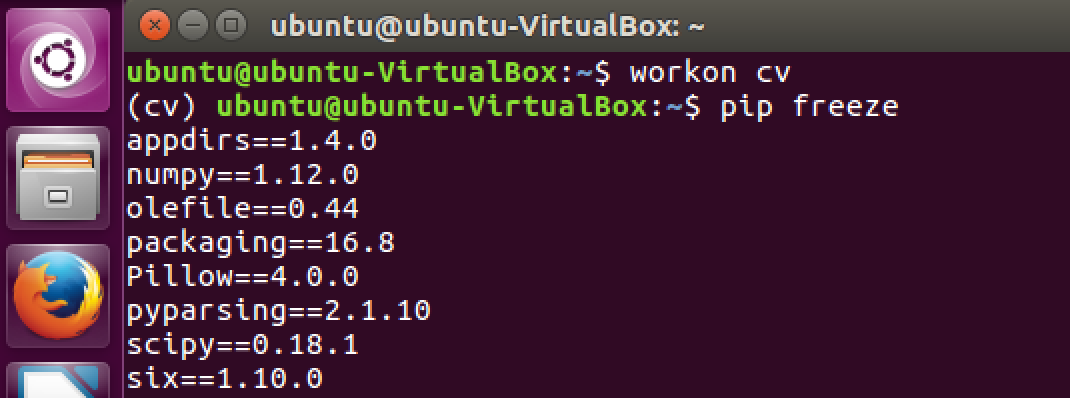
\includegraphics[width=15cm\textwidth]{pip-freeze}
    \caption{All the dependencies installed inside the virtualenv}
    \label{fig:virtual env pip freeze}
\end{figure}

In the above figure you can see all the python packages which are required for our project to function properly.

\subsection{Virtual Machine Architecture}

As we are running the whole experiment inside a virtual box, we have installed it behind MAC OSX. 

\begin{figure}[h]
    \centering
    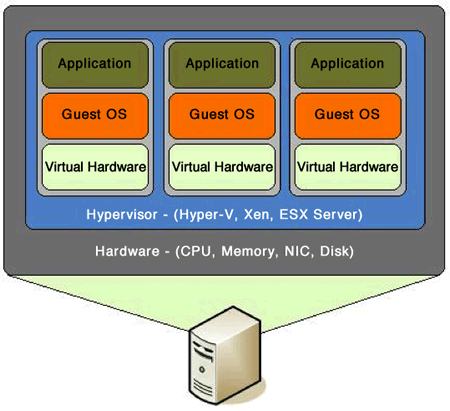
\includegraphics[width=12cm\textwidth]{virtual_machine}
    \caption{Virtual Machine architecture}
    \label{fig:virtual_machine_architecture}
\end{figure}

\subsection{Vagrant Virtual Environment}

Vagrant is a tool for building and managing virtual machine environments in a single workflow. With an easy-to-use workflow and focus on automation, Vagrant lowers development environment setup time, increases production parity, and makes the "works on my machine" excuse a relic of the past.

If you are already familiar with the basics of Vagrant, the documentation provides a better reference build for all available features and internals.

\subsubsection{Vagrant Architecture}

\begin{figure}[h]
    \centering
    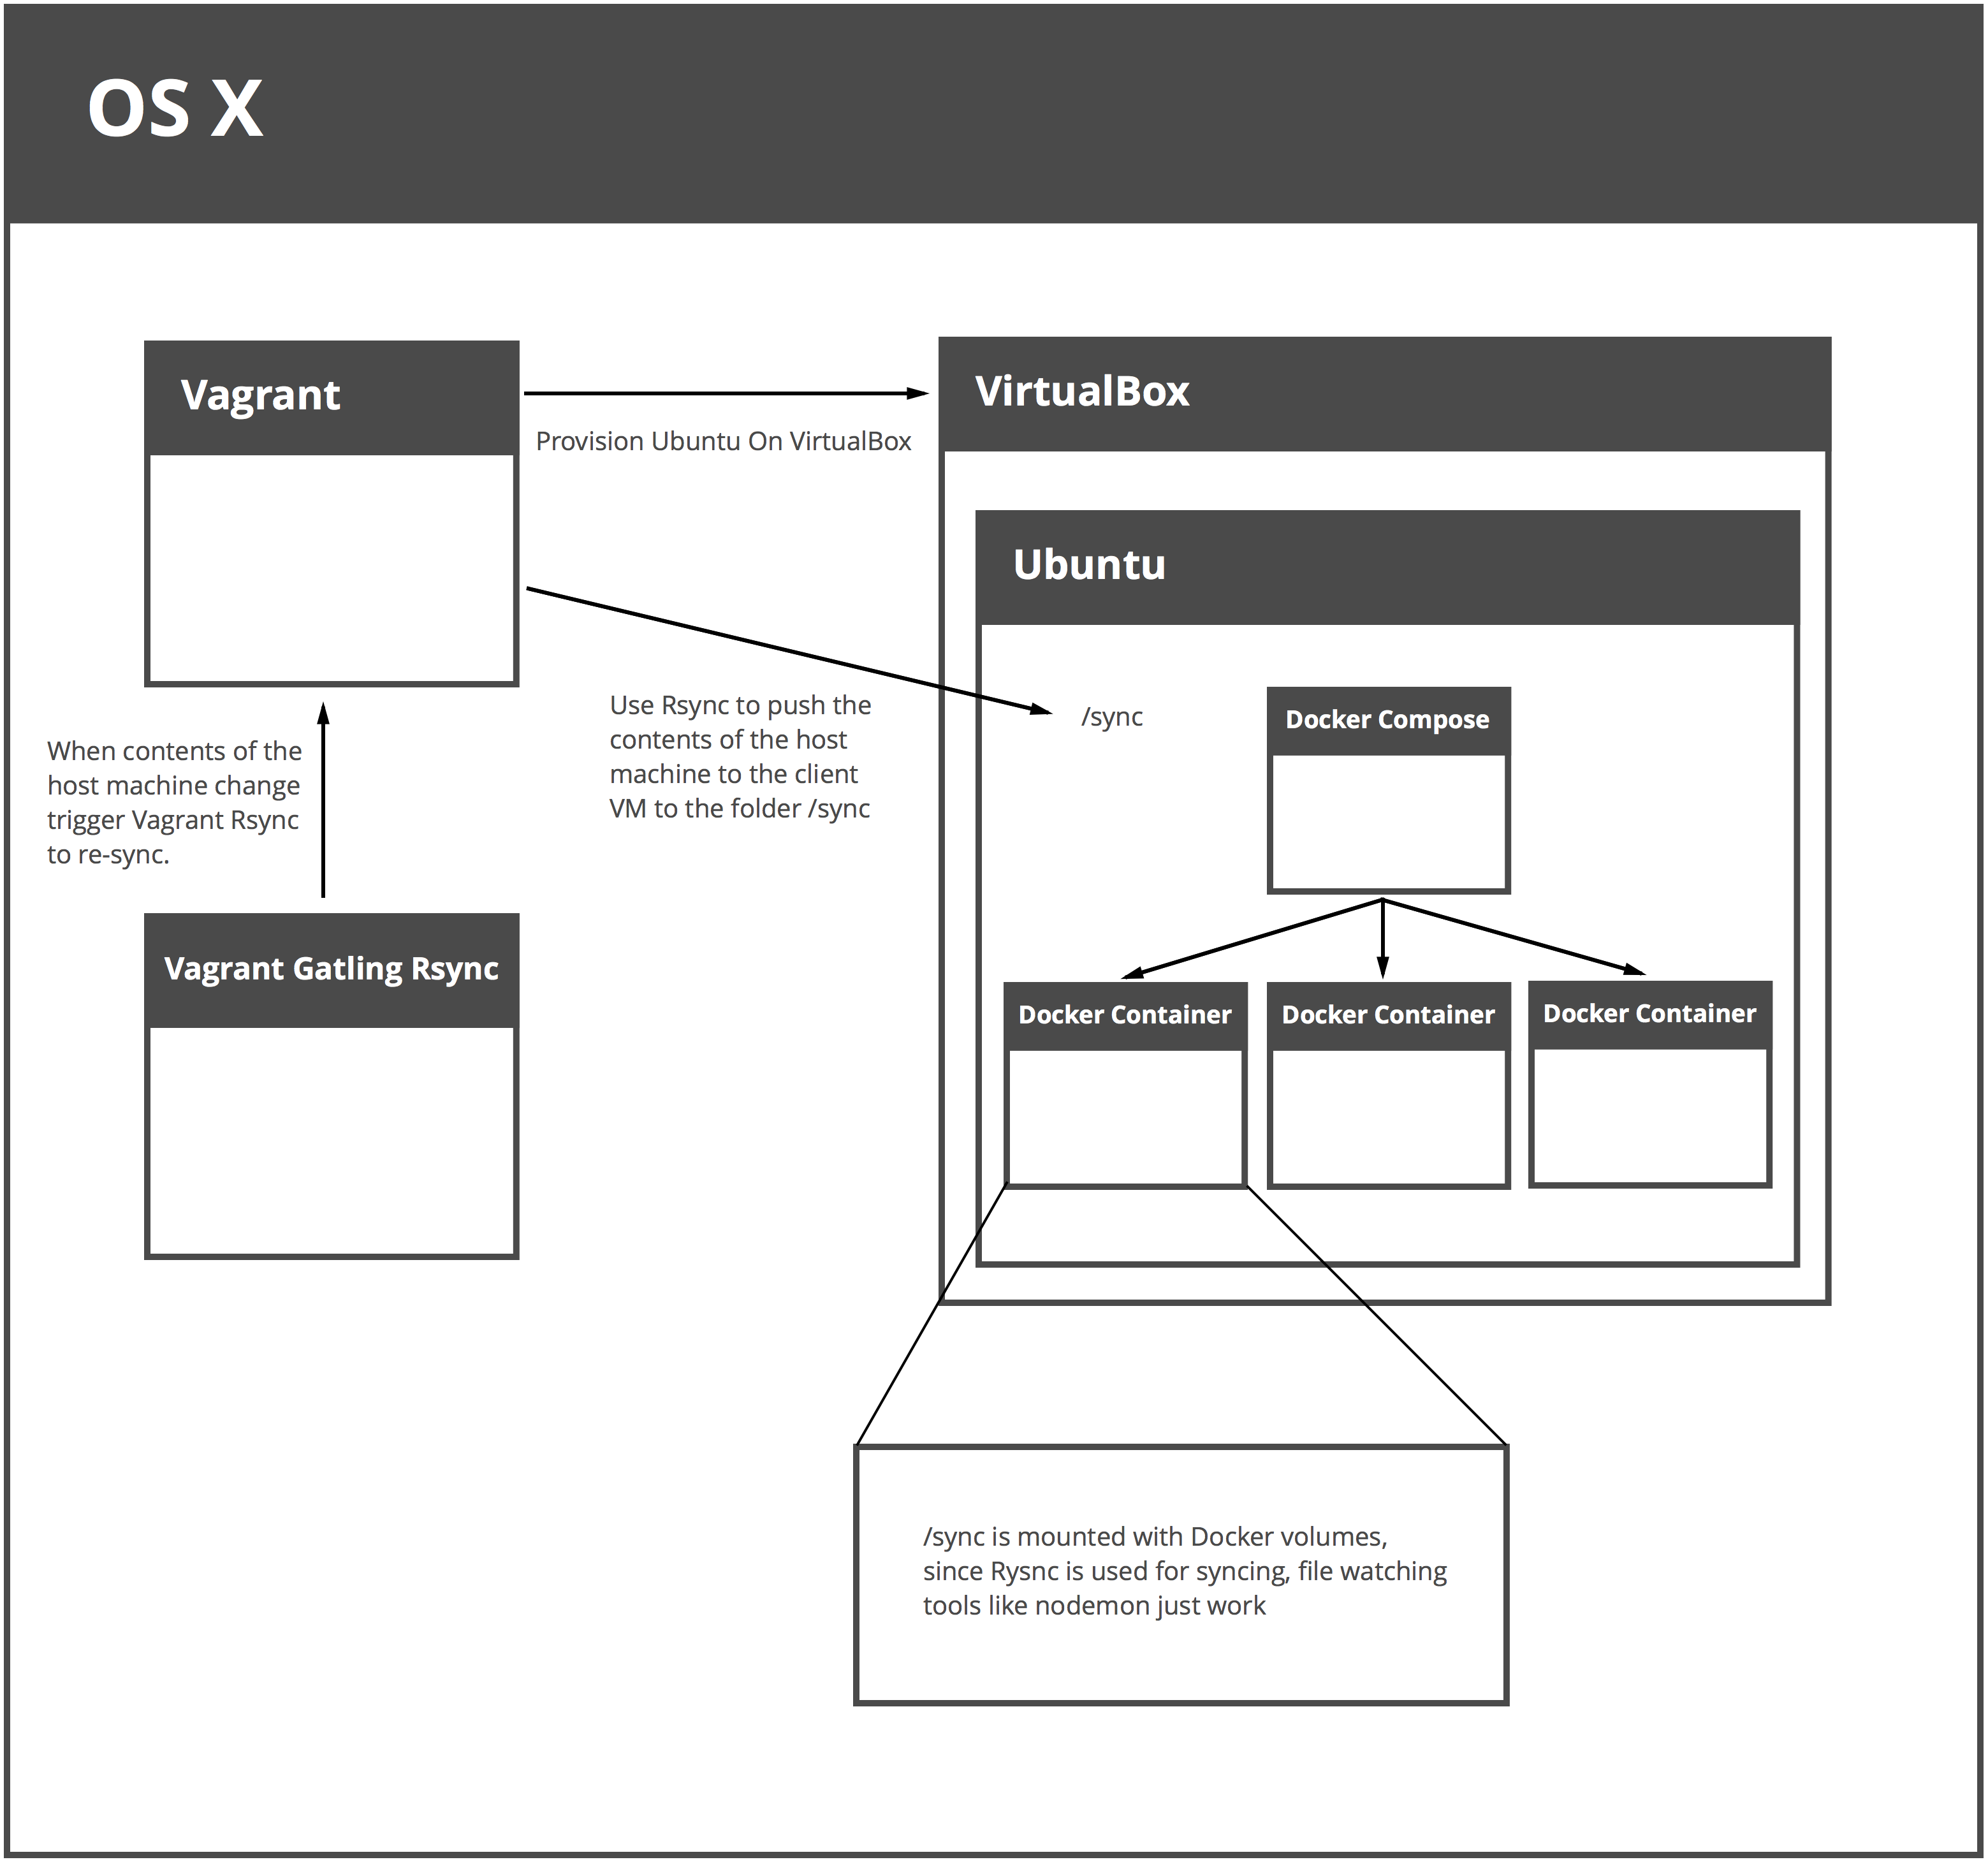
\includegraphics[width=12cm\textwidth]{vagrant-layers}
    \caption{Vagrant architecture in OSX}
    \label{fig:vagrant_arch}
\end{figure}

\subsubsection{Why Vagrant?}

Vagrant provides easy to configure, reproducible, and portable work environments built on top of industry-standard technology and controlled by a single consistent workflow to help maximize the productivity and flexibility of you and your team.

To achieve its magic, Vagrant stands on the shoulders of giants. Machines are provisioned on top of VirtualBox, VMware, AWS, or any other provider. Then, industry-standard provisioning tools such as shell scripts, Chef, or Puppet, can automatically install and configure software on the virtual machine.

If you are a developer, Vagrant will isolate dependencies and their configuration within a single disposable, consistent environment, without sacrificing any of the tools you are used to working with (editors, browsers, debuggers, etc.). Once you or someone else creates a single Vagrantfile, you just need to vagrant up and everything is installed and configured for you to work. Other members of your team create their development environments from the same configuration, so whether you are working on Linux, Mac OS X, or Windows, all your team members are running code in the same environment, against the same dependencies, all configured the same way. Say goodbye to "works on my machine" bugs.

\subsubsection{Advantages of developing with Vagrant}

\begin{enumerate}
    \item Set Up Multi-VM Networks with Ease
Most of the Vagrant power-user content I've read has been about setting up multiple VMs at the same time. Vagrant gives you a single config file to set these up, enabling you to launch all of them with one command.

Say you've configured three VMs to network with each other using static IPs on the 192.168.1.* subnet. You find yourself in a location that is already using that subnet to hand out IP addresses, and your VMs now conflict. With Vagrant, you can simply edit the Vagrantfile and reload the VMs, whereas with VirtualBox you'd have to open the settings for each VM, if not boot each VM and change them inside.

    \item Source Control
By putting the settings in a text file, it enables the configuration to be put under source control. Made some changes last week and accidentally broke the image? Just revert the changes and reload the VM. You can accomplish this with VirtualBox snapshots, but it will take up much more space than just a Vagrantfile.

    \item Various Platforms
This enables you to try various OSes or distributions, applying the same provisioning to set up similar environments. This can help with testing or adding support to new platforms, and would be time-consuming using just VirtualBox.
    
\end{enumerate}

% \subsubsection{Our Vagrantfile}
% as code should not be here

% \begin{lstlisting}[language=Ruby]
% # -*- mode: ruby -*-
% # vi: set ft=ruby :

% Vagrant.configure("2") do |config|    
%   config.vm.define "kurseve" do |server|
%     server.vm.box = "ubuntu/trusty64"
%     server.vm.hostname = "kurseve"
%     server.vm.provider "virtualbox" do |vb|
%       vb.memory = "2048"
%       vb.cpus = "2" 
%     end
%     server.ssh.insert_key = false
%     server.vm.provision "ansible" do |ansible|
%       ansible.verbose = "-vvv"
%       # If you want a less verbose one. Uncomment this.
%       # ansible.verbose = "-v"
%       ansible.playbook = "playbook.yml"
%     end
%   end
% end
% \end{lstlisting}
% % \lstinputlisting[language=Ruby]{Vagranfile.txt}

\subsection{Automation using Ansible}

\subsubsection{Introduction}

Ansible is a configuration management and provisioning tool, similar to Chef, Puppet or Salt.

I've found it to be one of the simplest and the easiest to get started with. A lot of this is because it's "just SSH"; It uses SSH to connect to servers and run the configured Tasks.

One nice thing about Ansible is that it's very easy to convert bash scripts (still a popular way to accomplish configuration management) into Ansible Tasks. Since it's primarily SSH based, it's not hard to see why this might be the case - Ansible ends up running the same commands.

We could just script our own provisioners, but Ansible is much cleaner because it automates the process of getting context before running Tasks. With this context, Ansible is able to handle most edge cases - the kind we usually take care of with longer and increasingly complex scripts.

Ansible Tasks are idempotent. Without a lot of extra coding, bash scripts are usually not safety run again and again. Ansible uses "Facts", which is system and environment information it gathers ("context") before running Tasks.

Ansible uses these facts to check state and see if it needs to change anything in order to get the desired outcome. This makes it safe to run Ansible Tasks against a server over and over again.

\subsubsection{Why Ansible?}

And, more generally, why use a configuration management tool at all? Anyone with an operations or development background have surely had to log into a server to change a configuration option, install a package, restart a service, or something else. It is easy enough to log in via SSH, make a quick change to get your application working, and then log out again. I know that I have done this hundreds (maybe thousands?) of times over my career. Sometimes, I would be diligent and document that change. More often, I would not. Then, weeks or months later, I would run into the same problem and have to rack my brain to remember how I fixed it. After resorting to scouring Google for answers, I’ll find the solution, slap my forehead, and then proceed to make the same exact change over again. This process may get you by for a time but there is definitely a better way. Especially in this day and age with the proliferation of cloud computing and cheap, disposable virtual machines, the ability to manage servers in a fast, repeatable and consistent manner is of paramount importance.

As mentioned above, there are a variety of tools that can help. But, there is definitely a barrier to entry, especially if you are just managing a handful of servers and don’t have the resources to spend a lot of time learning new tools. Chef and Puppet are fantastic and can be used to manage extremely large infrastructures but there is no denying that they have a large learning curve and can be difficult to setup and configure (at least in my experience). Ansible aims to be simpler and easier to understand while still maintaining the efficiency and power of other tools. It uses an agentless architecture so you don’t have to bootstrap your machines with a client application. And, it uses a simple configuration file format that is easy to understand and read for sysadmins and developers alike. Finally, Ansible unifies remote execution and configuration management - some other solutions require separate tools for these tasks. So, let’s take a look.

In order to follow along, you will need at least one server you can play around with. If you don’t have one, you can use Vagrant to spin up a virtual machine or two to work with. Another option I also like to use is DigitalOcean - it is an easy, low cost way to work with virtual machines in the cloud. You will also need a machine to run Ansible on. 

\subsubsection{Ansible YAML syntax}

For Ansible, nearly every YAML file starts with a list. Each item in the list is a list of key/value pairs, commonly called a “hash” or a “dictionary”. So, we need to know how to write lists and dictionaries in YAML.

There’s another small quirk to YAML. All YAML files (regardless of their association with Ansible or not) can optionally begin with --- and end with .... This is part of the YAML format and indicates the start and end of a document.

All members of a list are lines beginning at the same indentation level starting with a "- " (a dash and a space)

A dictionary is represented in a simple key: value form (the colon must be followed by a space)

Dictionaries and lists can also be represented in an abbreviated form if you really want to. YAML also supports dictionaries which map keys to values.

\subsubsection{Ansible Variables}

Variable names should be letters, numbers, and underscores. Variables should always start with a letter.

\begin{itemize}
    \item \detokenize{foo_port} is a great variable. foo5 is fine too.
    \item foo-port, foo port, foo.port and 12 are not valid variable names.
\end{itemize}

\subsubsection{Ansible Variable Scopes}

Ansible variable scopes are not that dissimilar from how scopes work and are understood in the general programming world.

Ansible has 3 main scopes:

\begin{itemize}
    \item Global: \par this is set by config, environment variables and the command line
    \item Play: \par each play and contained structures, vars entries, \detokenize{include_vars}, role defaults and vars.
    \item Host: \par variables directly associated to a host, like inventory, facts or registered task outputs

\end{itemize}

\subsubsection{Ansible Modules}

Modules are Ansible’s way of abstracting certain system management or configuration tasks. In many ways, this is where the real power in Ansible lies. By abstracting commands and state into modules, Ansible is able to make system management idempotent. This is an important concept that makes configuration management tools like Ansible much more powerful and safe than something like a typical shell script. It is challenging enough to write a shell script that can configure a system (or lots of systems) to a specific state. It is extremely challenging to write one that can be run repeatedly against the same systems and not break things or have unintended side effects. When using idempotent modules, Ansible can safely be run against the same systems again and again without failing or making any changes that it does not need to make.

There is a large catalog of modules available for Ansible out of the box. Here are just a very small sample of some things that can be managed with Ansible modules:

\begin{itemize}
    \item users
    \item groups
    \item packages
    \item and a lot more
\end{itemize}

If there is not a specific module available to accomplish a certain task, you can also just run arbitrary commands with Ansible or you can create your own custom module.

\subsubsection{Structuring your Ansible roles}

In order for Ansible to correctly handle roles, we need to build a directory structure that it can find and understand. We can do this by creating a "roles" directory in our working directory for Ansible.

There is a directory called "roles" inside the home directory where are the roles are separately put inside and organised, this helps in keeping things organised and modular.

These are the directories that will contain all of the code to implement our configuration. In real practice all may not be required 

\begin{figure}[h]
    \centering
    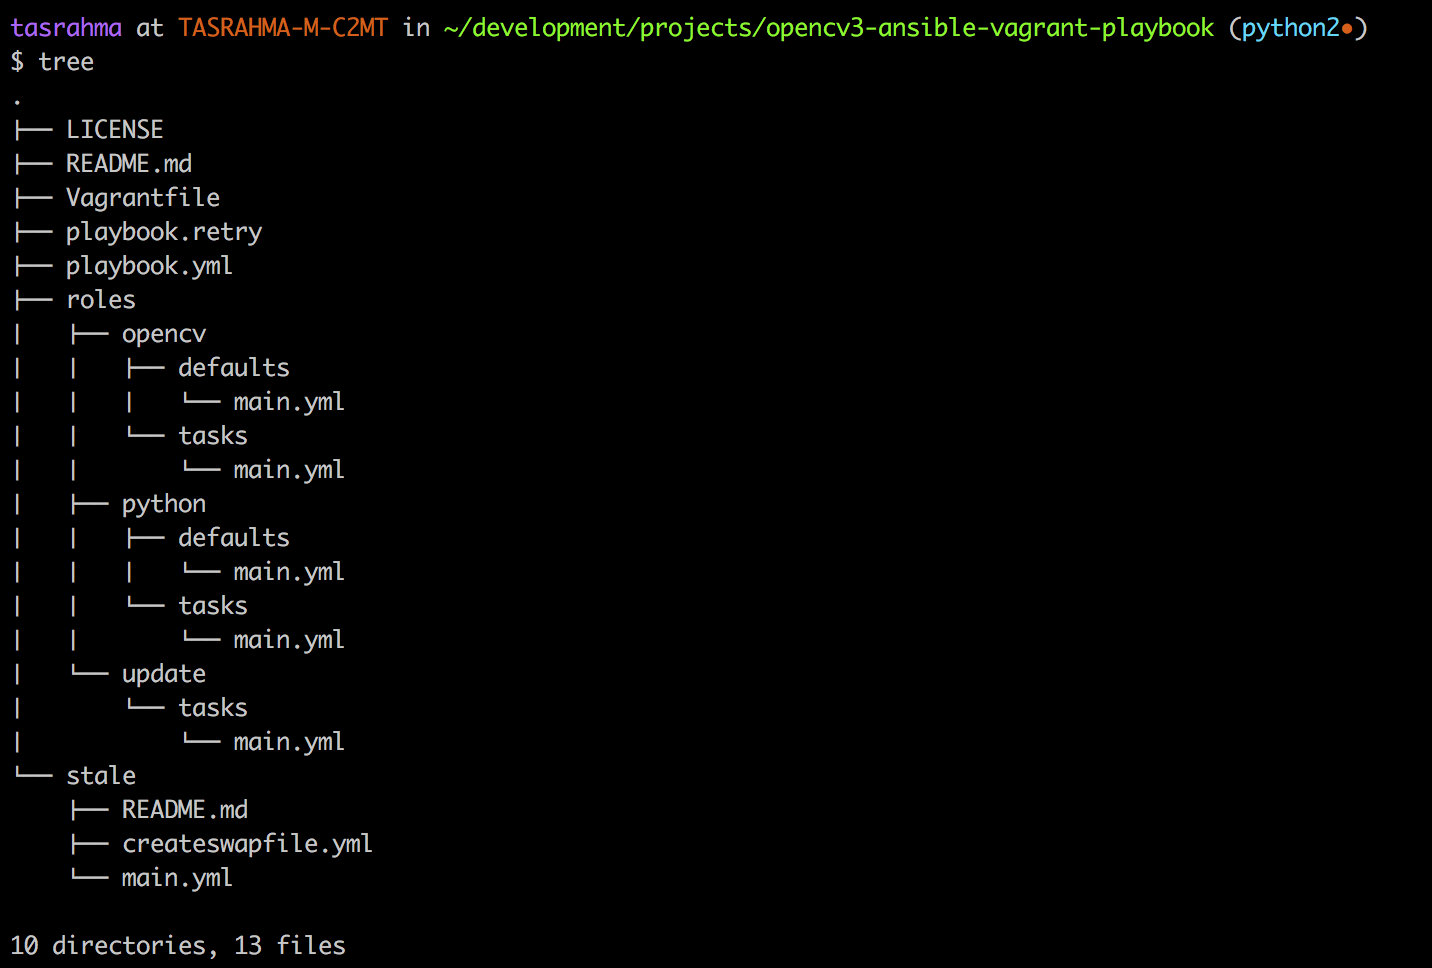
\includegraphics[width=15cm\textwidth]{opencv-ansible-play}
    \caption{Ansible Directory structuring}
    \label{fig:Ansible Directory structuring}
\end{figure}

This is what they are all for:

\begin{itemize}
    \item files: \par This directory contains regular files that need to be transferred to the hosts you are configuring for this role. This may also include script files to run.
    \item handlers: \par All handlers that were in your playbook previously can now be added into this directory.
    \item meta: \par This directory can contain files that establish role dependencies. You can list roles that must be applied before the current role can work correctly.
    \item templates: \par You can place all files that use variables to substitute information during creation in this directory.
    \item tasks: \par This directory contains all of the tasks that would normally be in a playbook. These can reference files and templates contained in their respective directories without using a path.
    \item vars: \par Variables for the roles can be specified in this directory and used in your configuration files.
\end{itemize}

Within all of the directories but the "files" and "templates", if a file called playbook.yml exists, its contents will be automatically added to the playbook that calls the role.

Ansible roles are an optional feature to take advantage of, but if you plan on using Ansible extensively, it is highly recommended that you explore this functionality. Not only will it keep your host-level configuration clean and readable, it will also allow you to easily reuse code and implement your changes in a modular fashion.

%%%%%%%%%%%%%%%%%%%%%%%%%%%%%%%%%%%%%%%%%%%%%%%%%%%%%%%%%%%%
\chapter{Implementation}

\section{Canny Edge}

\subsection{With a Dark Image}

\begin{figure}[h]
    \centering
    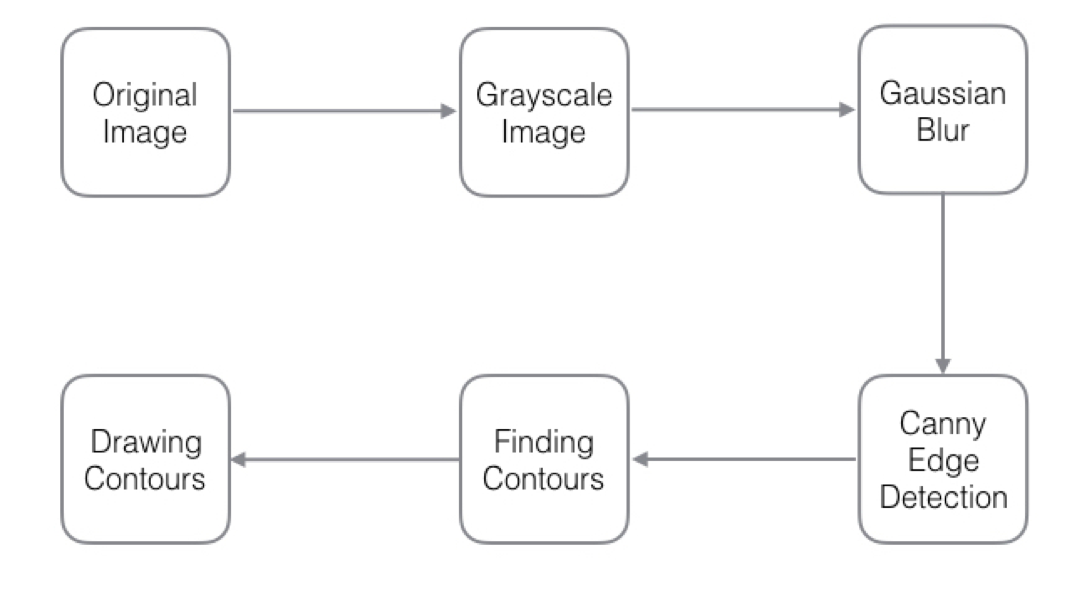
\includegraphics[width=16cm\textwidth]{canny_pipeline}
    \caption{Canny edge Pipeline}
    \label{fig:canny edge pipeline}
\end{figure}

We would be first trying out the canny edge detection algorithm on an image with a dark background.

The figure that you see above is the image processing pipeline that we have decided upon for canny edge detection process.

\newpage

\subsubsection{Original Image}

The very first thing to do is to load the image into memory from disk. We can load it off disk using the cv2.imread function from OpenCV. 

The cv2.imread function returns a NumPy array representing the image. Again, since images are represented as NumPy arrays.

\begin{figure}[h!]
    \centering
    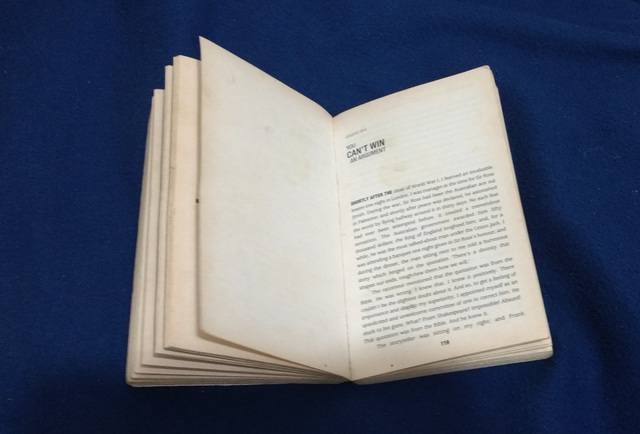
\includegraphics[width=15cm\textwidth]{canny-edge-in1}
    \caption{Canny edge original input image with uniform dark background}
    \label{fig:Canny edge input with uniform background}
\end{figure}

\subsubsection{Grayscale Image}

The next step in the pipeline is to grayscale the image which in which the value of each pixel is a single sample, that is, it carries only intensity information. Images of this sort, also known as black-and-white, are composed exclusively of shades of gray, varying from black at the weakest intensity to white at the strongest.

\begin{figure}[h!]
    \centering
    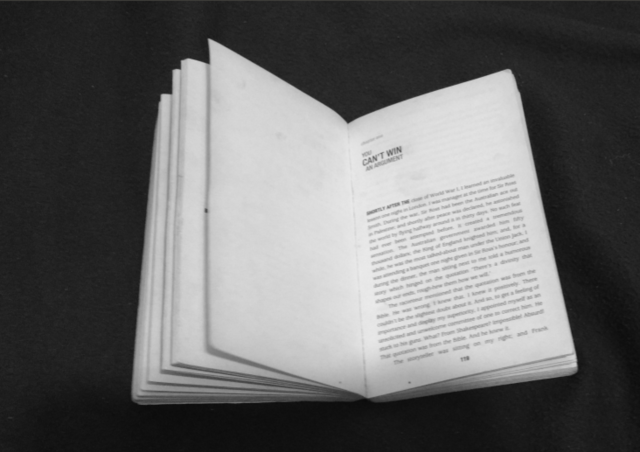
\includegraphics[width=15cm\textwidth]{win_frnds_blue_gray_640x480}
    \caption{Canny edge input with uniform dark background grayscaled}
    \label{fig:Canny edge input with uniform background grayscaled}
\end{figure}

\newpage

\subsubsection{Gaussian Blur}

Out of the many smoothening and blurring techniques used, we are going with gaussian blur here as it will be more effective in this certain situation than the other method.

It is a widely used effect in graphics software, typically to reduce image noise and reduce detail. The visual effect of this blurring technique is a smooth blur resembling that of viewing the image through a translucent screen, distinctly different from the bokeh effect produced by an out-of-focus lens or the shadow of an object under usual illumination. Gaussian smoothing is also used as a pre-processing stage in computer vision algorithms in order to enhance image structures at different scales—see scale space representation and scale space implementation.

\begin{figure}[h!]
    \centering
    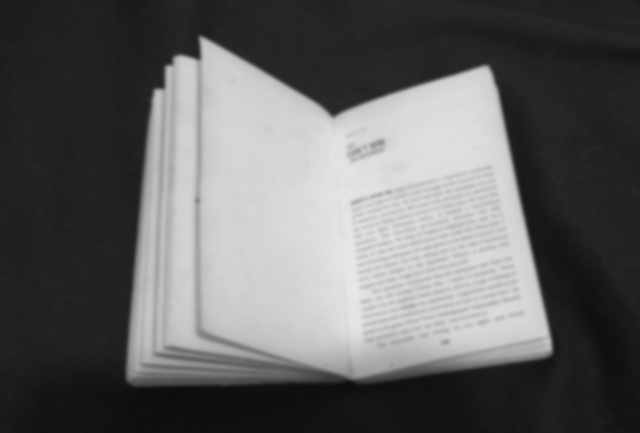
\includegraphics[width=15cm\textwidth]{win_frnds_blue_grayed_640_480}
    \caption{Canny edge input with uniform dark background grayscaled and blurred}
    \label{fig:Canny edge input with uniform background grayscaled}
\end{figure}

\newpage

\subsubsection{Canny Edge Detection}

Canny Edge detection algorithm is applied on the image which is received after a gaussian blur to it. Greyscaling the image before blurring it is used as a pre-processing technique to properly handle all the images and for gettin the best possible output.

\begin{figure}[h!]
    \centering
    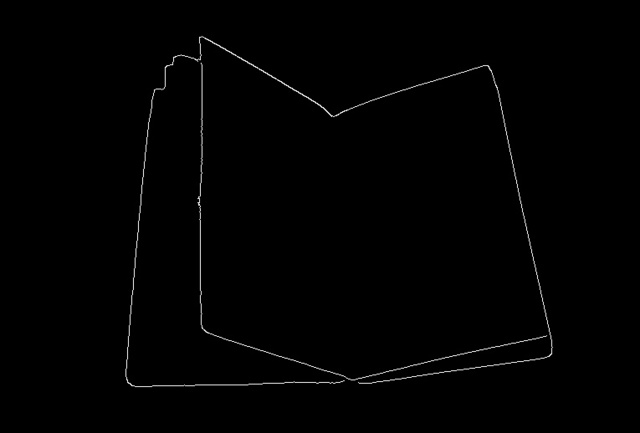
\includegraphics[width=15cm\textwidth]{win_frnds_blue_canny_640x480}
    \caption{Canny edge with uniform dark background edges}
    \label{fig:Canny edge input with uniform background edges}
\end{figure}

\subsubsection{Finding Contours}

This step involves finding the contours of our image. This means finding the edges on top of which the contours will be drawn using a custom color specified by us.

\subsubsection{Drawing Contours}

This step is where we draw the contours in a  color specified by us. This shows the borders or edges if you may in clear visuals.

It is the last step of the whole pipeline and as everything goes in a sequential manner. You can use any colors for drawing the contours.

For the purpose of this experiment, we used the green color to draw the contours.

\begin{figure}[h!]
    \centering
    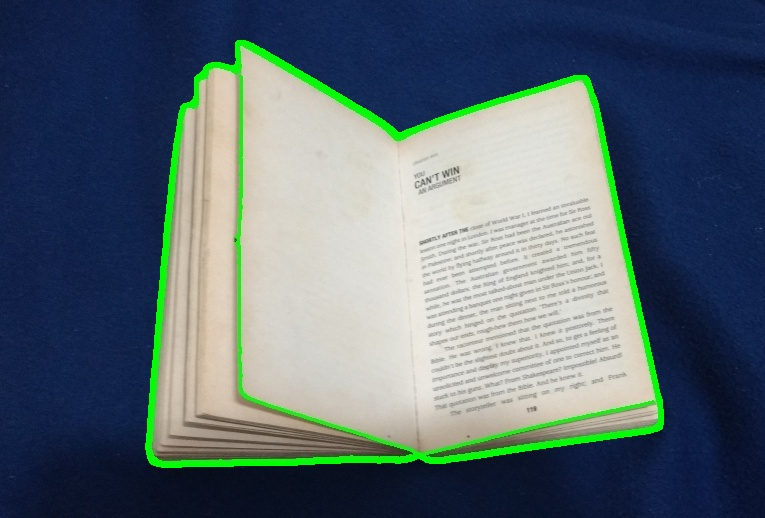
\includegraphics[width=15cm\textwidth]{canny-edge-out1}
    \caption{Canny edge output with uniform dark background}
    \label{fig:Canny edge output with uniform background}
\end{figure}

\newpage

\subsection{With Multi Colored background}

As we tried with a dark background in the previous section we are trying the experiment again with a multi-colored background image. 

This will help us test our accuracy for the image detection technique and help us compare it with sobel and laplace edge detection methods.

We are not trying this out with a light background as the accuracy when the background is very light, the algorithms are not able to detect the borders.

\newline

\begin{figure}[h!]
    \centering
    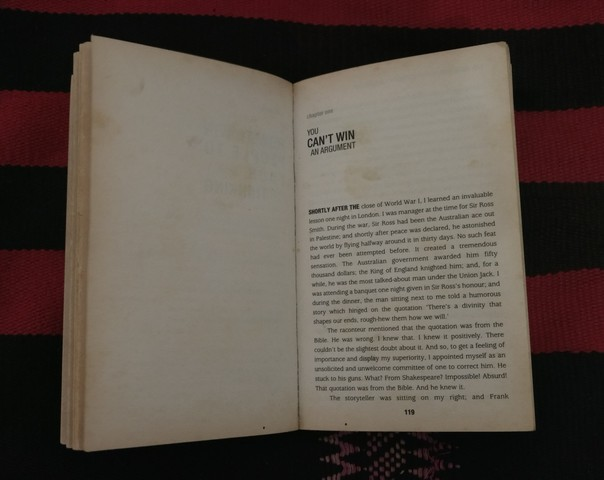
\includegraphics[width=15cm\textwidth]{canny-edge-in2}
    \caption{Canny edge input with multi-coloured background}
    \label{fig:Canny edge input with multi-coloured background}
\end{figure}

\newpage

When we follow the whole Image processing pipeline, we are getting a pretty efficient output for our input image.

\newline

\begin{figure}[h!]
    \centering
    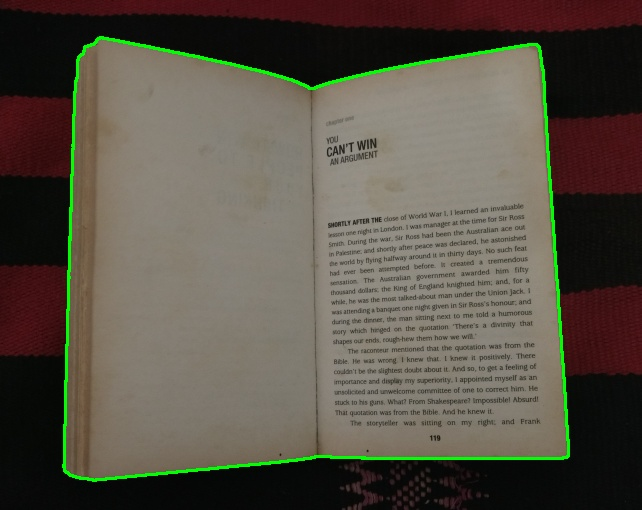
\includegraphics[width=15cm\textwidth]{canny-edge-out2}
    \caption{Canny edge output with multi-coloured background}
    \label{fig:Canny edge output with multi-coloured background}
\end{figure}

In the next section, we will try out the other edge detection techniques like

\begin{itemize}
    \item laplace
    \item sobel
\end{itemize}

And try to compare the methods which will help you best choose which algorithm to use for your image processing needs.

\newpage

\section{Laplace and Sobel}

\begin{figure}[h]
    \centering
    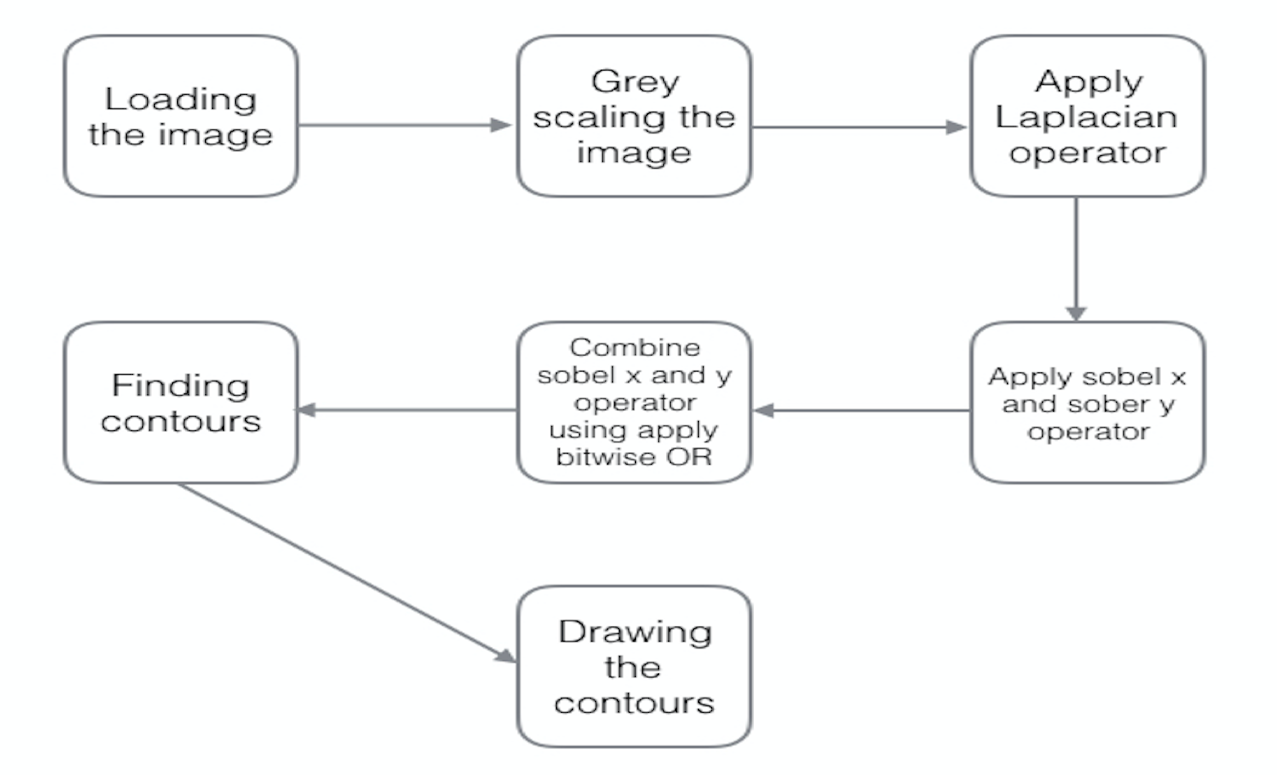
\includegraphics[width=17cm\textwidth]{laplace_and_sobel_pipeline}
    \caption{Laplace and Sobel Pipeline}
    \label{fig:laplace_and_sobel_pipeline}
\end{figure}

Sobel operators is a joint Gausssian smoothing plus differentiation operation, so it is more resistant to noise. You can specify the direction of derivatives to be taken, vertical or horizontal (by the arguments, y-order and x-order respectively). 

You can also specify the size of kernel by the argument ksize. If ksize = -1, a 3x3 Scharr filter is used which gives better results than 3x3 Sobel filter.

Using the Sobel operator, we can compute gradient magnitude representations along the x and y axis, allowing us to find both horizontal and vertical edge-like regions.

\begin{figure}[h!]
    \centering
    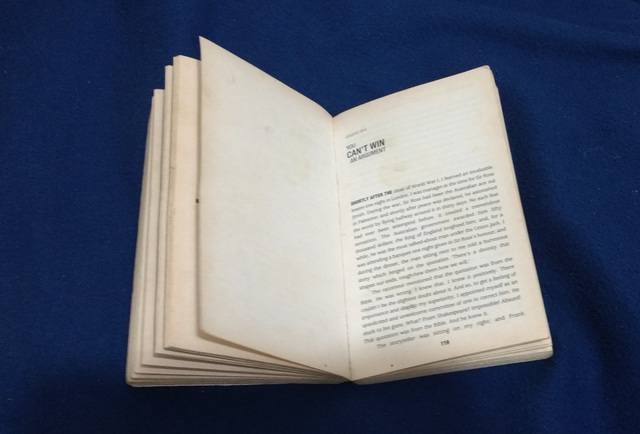
\includegraphics[width=15cm\textwidth]{canny-edge-in1}
    \caption{Laplace-Sobel input with uniform dark background}
    \label{fig:Laplace & Sobel input with uniform dark background}
\end{figure}

\subsection{Laplace operator}

Laplacian filters are derivative filters used to find areas of rapid change (edges) in images. Since derivative filters are very sensitive to noise, it is common to smooth the image (e.g., using a Gaussian filter) before applying the Laplacian. 

This two-step process is call the Laplacian of Gaussian (LoG) operation. There are different ways to find an approximate discrete convolution kernal that approximates the effect of the Laplacian.

The LoG operator takes the second derivative of the image. Where the image is basically uniform, the LoG will give zero. Wherever a change occurs, the LoG will give a positive response on the darker side and a negative response on the lighter side. At a sharp edge between two regions, the response will be

\begin{itemize}
    \item zero away from the edge
	\item positive just to one side
	\item negative just to the other side
	\item zero at some point in between on the edge itself
\end{itemize}
 
When using the filter given above, or any other similar filter, the output can contain values that are quite large and may be negative, so it is important to use an image type that supports negatives and a large range, and then scale the output. (ImageJ has a 32-bit floating point representation). Alternatively, a scaling factor can be used on the filter to restrict the range of values.

\begin{figure}[h!]
    \centering
    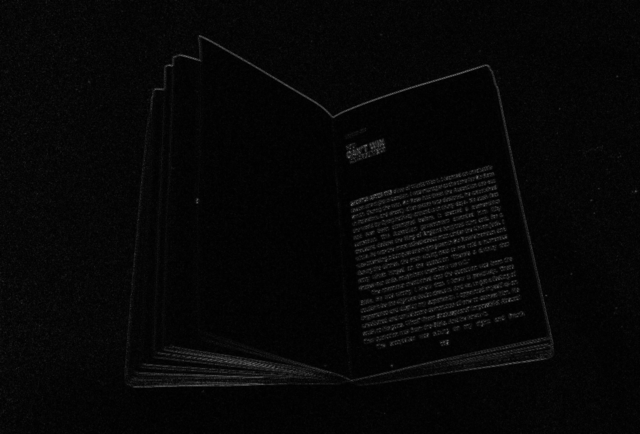
\includegraphics[width=15cm\textwidth]{laplace_640x480}
    \caption{Laplacian's output with uniform dark background}
    \label{fig:Laplacian's output with uniform dark background}
\end{figure}

\subsection{Sobel Operator}

The Sobel operator, sometimes called the Sobel–Feldman operator or Sobel filter, is used in image processing and computer vision, particularly within edge detection algorithms where it creates an image emphasising edges. It is named after Irwin Sobel and Gary Feldman, colleagues at the Stanford Artificial Intelligence Laboratory (SAIL). 

It was co-developed with Gary Feldman at SAIL. Sobel and Feldman presented the idea of an "Isotropic 3x3 Image Gradient Operator" at a talk at SAIL in 1968. Technically, it is a discrete differentiation operator, computing an approximation of the gradient of the image intensity function.

At each point in the image, the result of the Sobel–Feldman operator is either the corresponding gradient vector or the norm of this vector. 

Using the Sobel operator, we can compute gradient mag-
nitude representations along the x and y axis, allowing us to find both horizontal and vertical edge-like regions.

\subsection{Gradient in X-Axis}

\begin{figure}[h!]
    \centering
    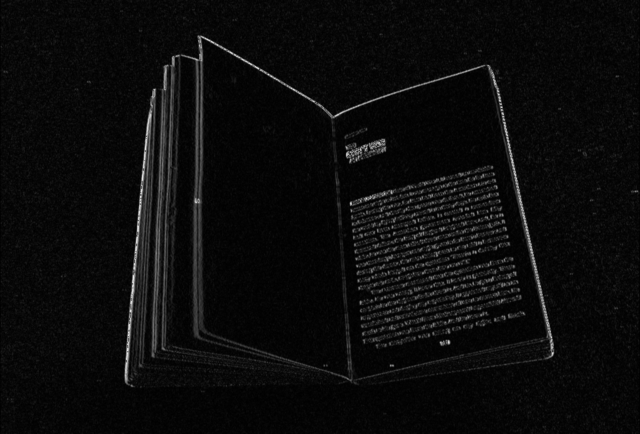
\includegraphics[width=13.5cm\textwidth]{sobelx_640x480}
    \caption{Sobel's x-axis output with uniform dark background}
    \label{fig:Sobel's x-axis output with uniform dark background}
\end{figure}

\subsection{Gradient in Y-Axis}

\begin{figure}[h!]
    \centering
    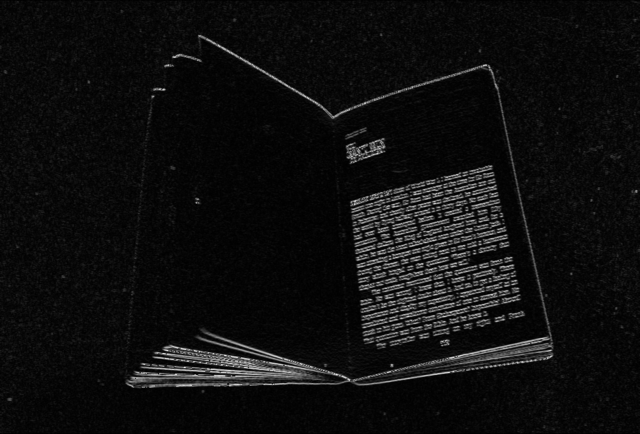
\includegraphics[width=13.5cm\textwidth]{sobely_640x480}
    \caption{Sobel's y-axis output with uniform dark background}
    \label{fig:Sobel's y-axis with uniform dark background}
\end{figure}


\newpage

\subsection{Combined Gradient of XY-Axis}

In order to combine the gradient images in both the x and y direction, we can apply a bitwise OR. Remember, an OR operation is true when either pixel is greater than zero. 

Therefore, a given pixel will be True if either a horizontal or vertical edge is present.

\begin{figure}[h!]
    \centering
    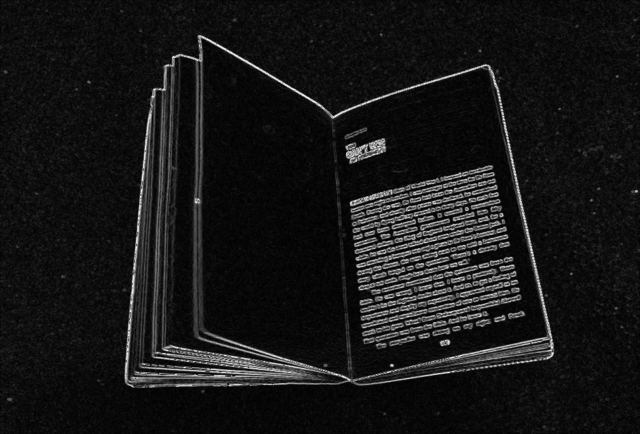
\includegraphics[width=15cm\textwidth]{sobel_xy_combined_640x480}
    \caption{Sobel's x and y-axes combined output with uniform dark background}
    \label{fig:Sobel's x and y-axes combined output with uniform dark background}
\end{figure}

As you can see, the combined XY-Axis output is much more sharper and clearer than the individual X-axis gradient and the Y-Axis gradient.

\section{Combined Sobel and Laplace Operator}

Here we are trying to combine both the 

\begin{itemize}
    \item Laplace operator
    \item Sobel Operator
\end{itemize}

So first, we are passing the greyscaled and blurred image to the Laplacian operator and then after that we are passing the output of the laplacian operator to the Sobel operator as input. 

\begin{figure}[h!]
    \centering
    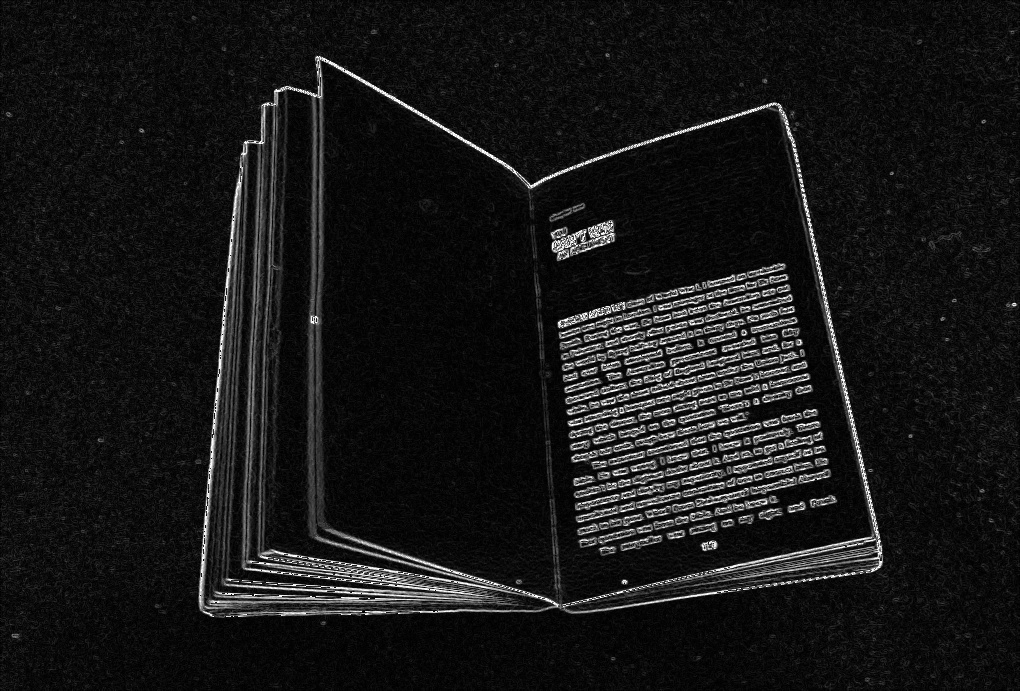
\includegraphics[width=15cm\textwidth]{sobel-out}
    \caption{Laplace-Sobel output with uniform dark background}
    \label{fig:Laplace & Sobel output with uniform dark background}
\end{figure}

The end result is much clearer to detect the edges from from the previous combined XY-Axix Sobel operator.

\section{Comparison of Number of edges detected correctly}

\begin{figure}[h!]
    \centering
    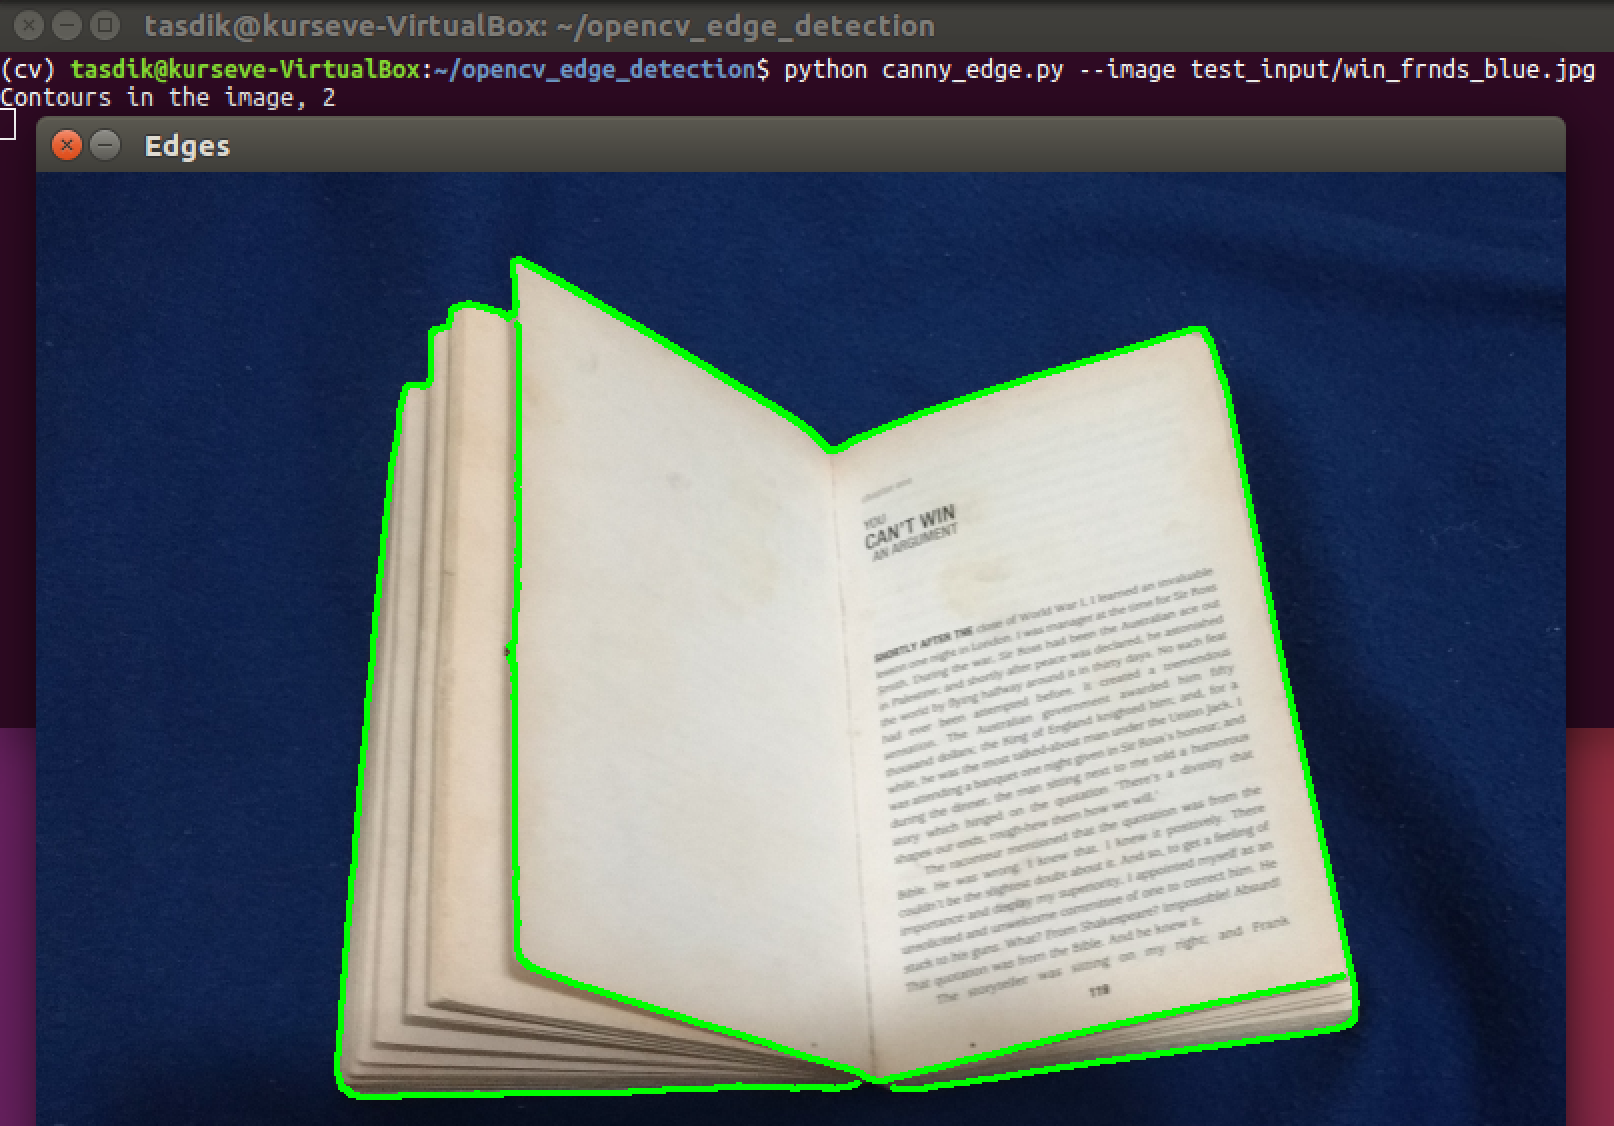
\includegraphics[width=15cm\textwidth]{number_of_edges_canny}
    \caption{Number of Edges detected by Canny Edge on input images}
    \label{fig:Number of Edges detected by canny on input images}
\end{figure}

We give the algorithms the same test image as input. And from our experiment results observe that in comparison to Canny Edge (in figure \ref{fig:Number of Edges detected by canny on input images}), Laplace and Sobel are not able to detect the number of edges properly in the test input image (in figure \ref{fig:Number of Edges detected by Laplace and Sobel on input images})

\begin{itemize}
    \item Canny Edge: Able to detect the two edges correctly
    \item Sobel and Laplace: Detects one edge
\end{itemize}

\begin{figure}[h!]
    \centering
    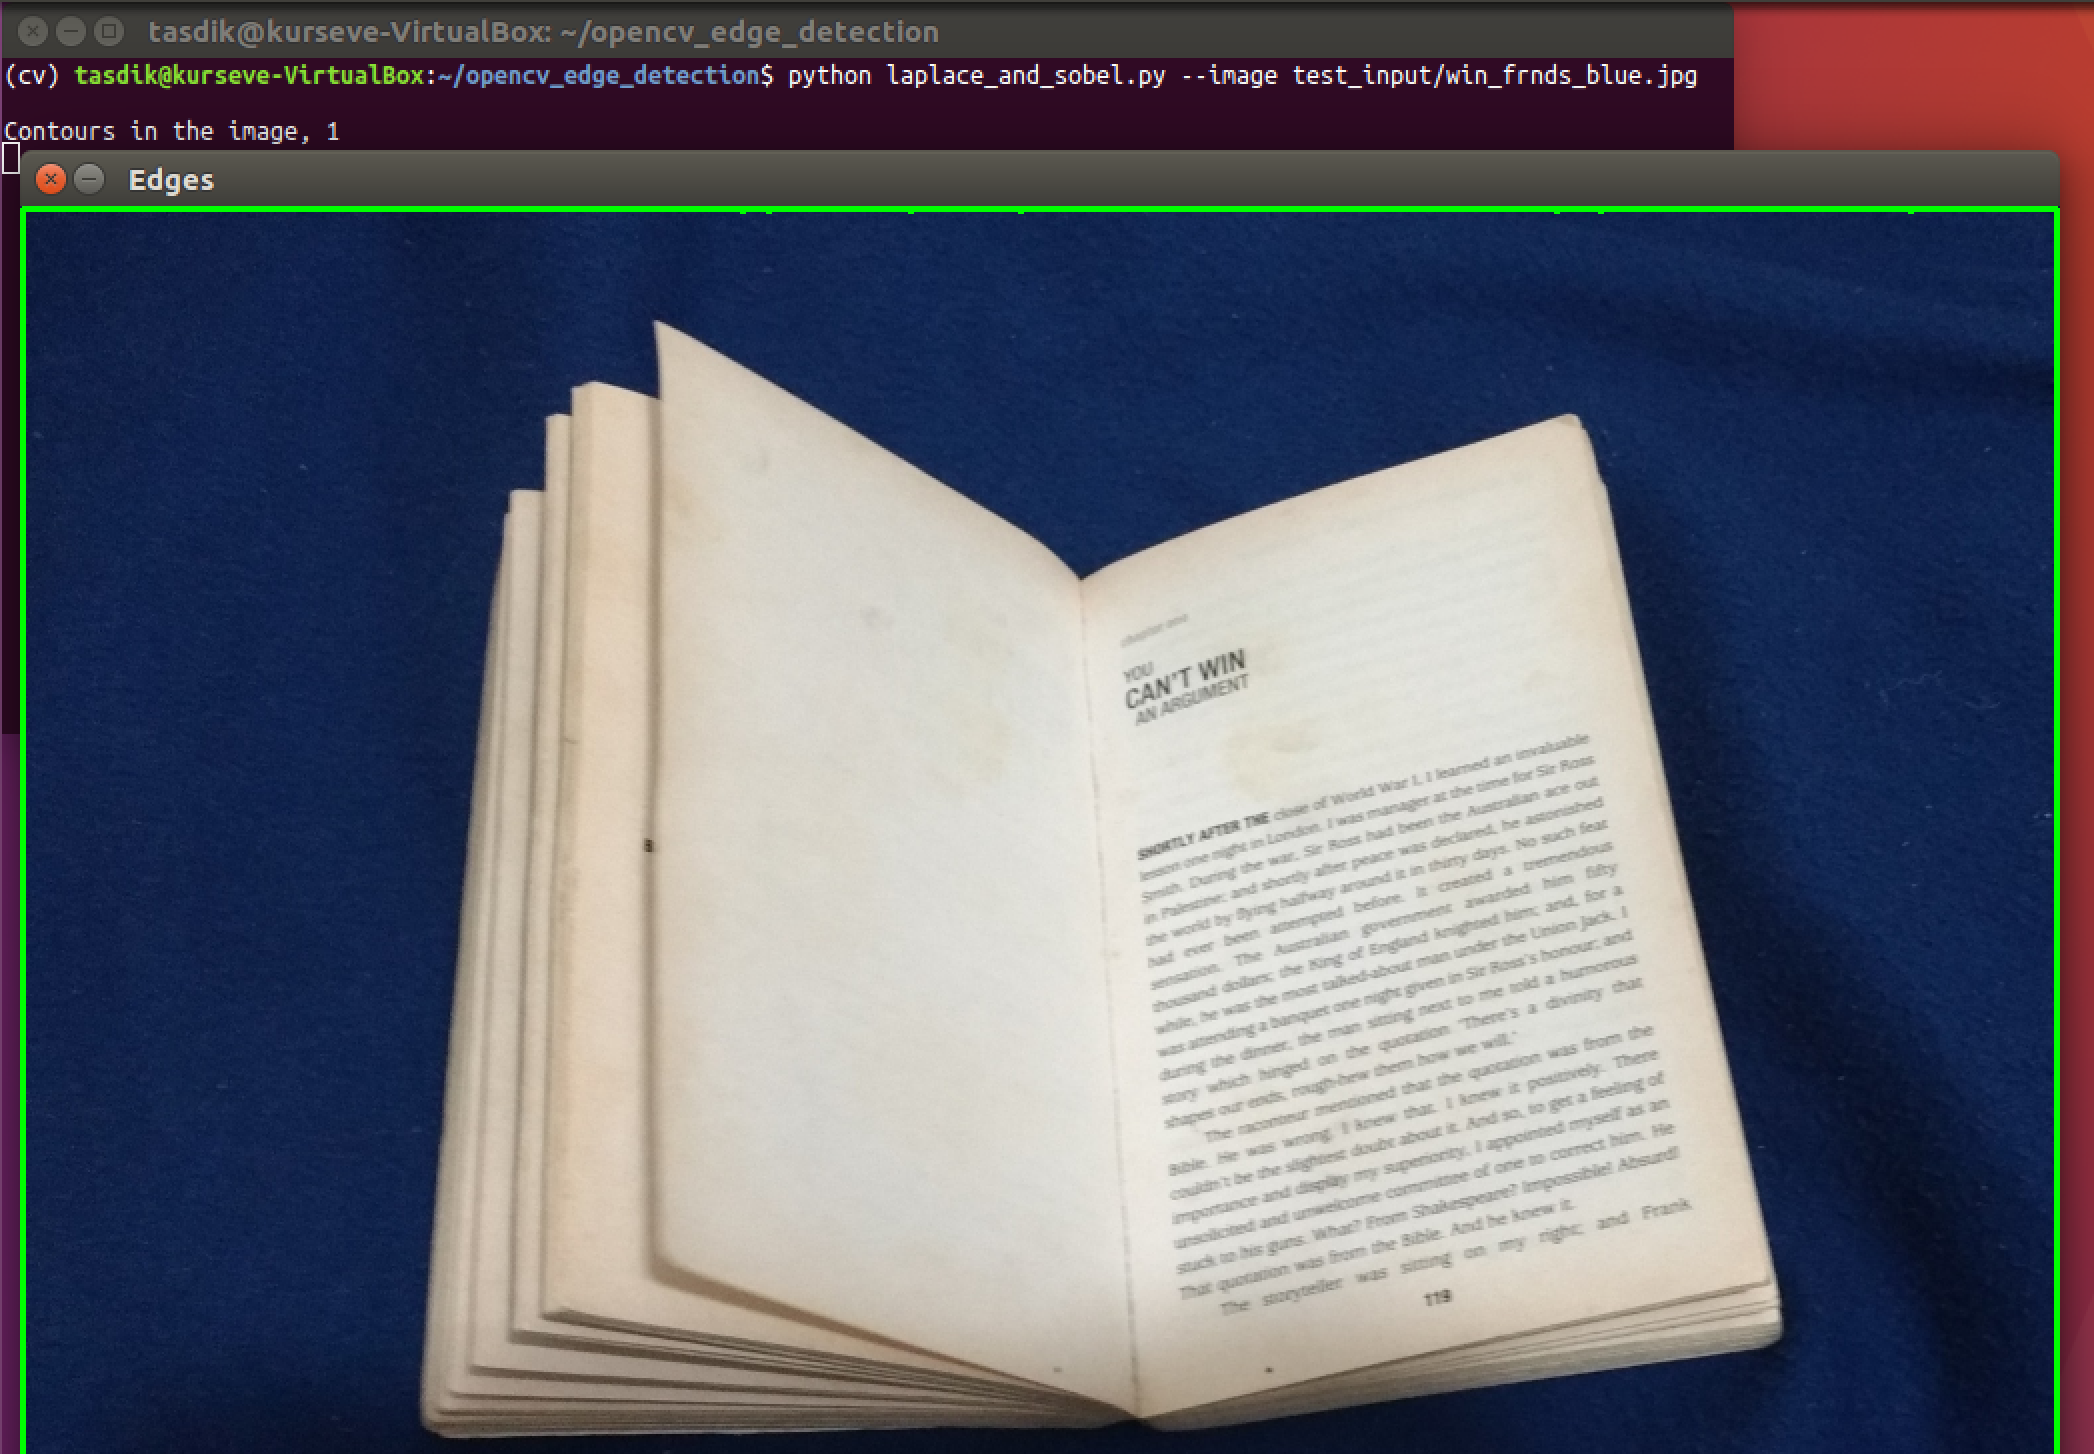
\includegraphics[width=15cm\textwidth]{number_of_edges_laplace_sobel}
    \caption{Number of Edges detected by Laplace and Sobel on input images}
    \label{fig:Number of Edges detected by Laplace and Sobel on input images}
\end{figure}


%%%%%%%%%%%%%%%%%%%%%%%%%%%%%%%%%%%%%%%%%%%%%%%%%%%%%%%%%%%%
\chapter{Conclusion}
In this project on different popular methods of Image Processing, our survey dives deeper into comparing some of the most used methods of edge detection especially in the case of textual notes. 

From the above findings, it can be said that the Canny Edge Detection method with its multi-stage nature works best on most images which require edge detection and gradient analysis while Laplace and Sobel method can be pretty helpful for application with much simpler image manipulation operations.

\chapter{Result}
In this particular project on processing images of textual notes or documents is one of many scenarios where Computer Vision can aid in better understand the various methods to improve upon the readability and enable better archives of digital documents. 


Here have demonstrated how Canny Edge detection proves to be superior for edge extraction from notes and documents over other popular methods of edge detection, namely Laplace and Sobel Edge detection techniques. 

This experiment is aimed to aid in finding a best fitting algorithm or technique while detecting edges in everyday photos of textual documents and notes.

\chapter{Future Enhancement}
This project is done based on the most popular edge detection techniques found in articles and code bases with similar work done in the area.

In our project, we have mainly narrowed down our focus onto three main edge detection algorithms or techniques, namely Laplace, Sobel and Canny edge detection.There are several other capable algorithms and techniques to detect edges in images of notes and other literature material that have in someway lost detail and no longer retain full readability as earlier.

Some other methods that could also serve this purpose in resolving digital images of notes and documents are as follows:
\begin{enumerate}
    \item Robert's edge detector
    \item Prewitt edge detector
    \item Frie Chen edge detector
\end{enumerate}

These methods of edge detection could prove to be vital in certain cases of edge detection that has not been covered in this project. Since all of these edge detection techniques have slightly different approaches, therefore their outcomes vary in terms of amount of noise that they can filter out and the accuracy in number of actual edges detected that may be what a particular experiment or project requires. It is always about selecting the best possible approach that would fit best for that particular purpose.

%%%%%%%%%%%%%%%%%%%%%%%%%%%%%%%%%%%%%%%%%%%%%%%%%%%%%%%%%%%%
% Appendices.

\appendix
\chapter{VECTOR ALGEBRA}
\section{Product of Two Vectors}
\label{app:vp}
The product of two vectors are may be a scalar product or vector product. The scalar product of two vectors is also called as dot product. It is defined as $\vec{a} . \vec{b}=|\vec{a}||\vec{b}|cos\theta$ where $\theta$ is the angle between the two vectors $\vec{a}$ and $\vec{b}$

The cross product or vector product is a binary operation on two vectors in three-dimensional space and is denoted by the symbol $\times$. The cross product $\vec{a}\times\vec{b}$ of two linearly independent vectors $\vec{a}$ and $\vec{b}$ is a vector that is perpendicular to both and therefore normal to the plane containing them. 
\chapter{MATRIX ALGEBRA}
\section{Matrix Multiplication}
Matrix multiplication \footnote{\url{https://en.wikipedia.org/wiki/Canny_edge_detector#Development_of_the_Canny_algorithm}} is a binary operation that takes a pair of matrices, and produces another matrix. Numbers such as the real or complex numbers can be multiplied according to elementary arithmetic. On the other hand, matrices are arrays of numbers, so there is no unique way to define multiplication of matrices. As such, in general the term ``matrix multiplication'' refers to a number of different ways to multiply matrices. 

%%%%%%%%%%%%%%%%%%%%%%%%%%%%%%%%%%%%%%%%%%%%%%%%%%%%%%%%%%%%
% Code

\chapter{Code}
\section{Canny edge}

\subsection{Edge Detection}

\lstinputlisting[language=Python]{source_code/canny_edge.py}

\subsection{Histogram}

\lstinputlisting[language=Python]{source_code/canny_edge_histogram.py}

\section{Laplace and sobel}

\subsection{Edge Detection}

\lstinputlisting[language=Python]{source_code/laplace_and_sobel.py}

\subsection{Histogram}

\lstinputlisting[language=Python]{source_code/laplace_and_sobel_histogram.py}



%%%%%%%%%%%%%%%%%%%%%%%%%%%%%%%%%%%%%%%%%%%%%%%%%%%%%%%%%%%%
% Bibliography.

% \begin{singlespace}
%  \bibliography{thesis_refer} % Enter your .bib file name here
% \end{singlespace}
%%%%%%%%%%%%%%%%%%%%%%%%%%%%%%%%%%%%%%%%%%%%%%%%%%%%%%%%%%%%

% REF: http://kb.mit.edu/confluence/pages/viewpage.action?pageId=3907111

  \begin{thebibliography}{1}

  \bibitem{into_image_processing_sisu} University of Tartu, {\em Introduction to image processing, 2014}
  \newline
  \url{https://sisu.ut.ee/imageprocessing/book/1}
  
  \bibitem{wiki_image_processing}Wikipedia, {\em Image processing}
  \newline
  \url{https://en.wikipedia.org/wiki/Image_processing}
  
  \bibitem{wiki_digital_image_processing}Wikipedia, {\em Digital Image processing}
  \newline
  \url{https://en.wikipedia.org/wiki/Digital_image_processing}
  
   \bibitem{wiki_edge_detection}Wikipedia, {\em Edge Detection}
  \newline
  \url{https://en.wikipedia.org/wiki/Edge_detection}

   \bibitem{researchgate_edge_det} Researchgate, {\em Edge Detection Techniques for Image
Segmentation – A Survey of Soft Computing Approaches}
   \newline
   \url{https://www.researchgate.net/profile/Reghunadhan_Rajesh/publication/228349759_Edge_Detection_Techniques_for_Image_Segmentation_-_A_Survey_of_Soft_Computing_Approaches/links/0912f50a60060decac000000.pdf}

   \bibitem{drexel_canny}Drexel university, {\em Canny edge detection}
   \newline
   \url{http://www.pages.drexel.edu/~nk752/Research/cannyTut2.html}
   
   \bibitem{austin_g_walters} Austin G. Walters, {\em Edge Detection in Computer Vision}
   \newline
   \url{http://austingwalters.com/edge-detection-in-computer-vision/}
   
   \bibitem{ualberta_cs} University of Alberta, {\em Edge Detection}
   \newline
   \url{https://webdocs.cs.ualberta.ca/~nray1/CMPUT615_2010/Introduction/Edges.pdf}
   
   \bibitem{vipul-sharma} Vipul Sharma, {\em Sharingan:Tool to extract news articles from newspaper and give the context about the news}
   \newline
   \url{http://www.vipul.xyz/2017/03/sharingan-newspaper-text-and-context.html}
   
   \bibitem{elder_zucker_edge_detection} Elder Zucker,{\em Local scale control for edge detection and blur estimation, IEEE Transactions on Pattern Analysis and Machine Intelligence, vol. 20, no. 7, 699-716, 1998}
    
    \bibitem{linderberg_edge_detection} Tony Lindeberg,{\em Edge Detection and Ridge
Detection with Automatic Scale Selection, International Journal of Computer Vision 30(2): 117-156,1998}
    

  \end{thebibliography}
  \end{document}